% BangorEE - (an unofficial) Electronic Engineering Dissertation LaTeX Class.
% Usage info and bug reports at https://github.com/owenjones/bangoree

\documentclass[msc]{bangoree}

\usepackage{lipsum} % To create some filler content
\usepackage[style=authoryear-ibid]{biblatex}
\usepackage{amsmath}
\usepackage{subcaption}
\usepackage{appendix}

\title{Leksis: Prawf Geirfa Ymaddasol Am Ieithoedd Cyfyngedig eu Hadnoddau}
\author{Alan Kersaudy}
\course{Technoleg Iaith}
\date{Medi, 2025}
\supervisor{Dr.~G.~Bovolenta}

\addbibresource{references.bib}
\renewcommand{\appendixname}{Atodiad}
\makeatletter
\renewcommand{\@chapapp}{Pennod}
\makeatother

\begin{document}
    \maketitle
    \statements
    \abstract{abc}
    \cydnabyddion{\lipsum[1]}
    \tables

    \content
    \chapter{Cyflwyniad}    
\abbrv{IAC}{Ieithoedd Adnoddau Cyfyngedig}
Mae'r bennod gyntaf hon yn cyflwyno'r cyd-destun, a phwrpas y traethawd hir hwn. Yn benodol, daw'r drydedd adran â'r rôl y sydd gan dechnolegau addysgol i'w chwarae i'r amlwg, naill ai wrth gefnogi neu beryglu ymhellach Ieithoedd Adnoddau Cyfyngedig (IAC), yn dibynnu ar ai yw'r dechnoleg yn cael ei chynllunio i ddysgu ieithoedd sydd eisoes yn bygwth ieithoedd eraill. Gellir darllen yr adran hon fel cyflwyniad cyffredinol i faes technolegau addysgol i'r rhai hynny sy'n pryderu ynghylch tynged ieithoedd adnoddau cyfyngedig, neu fel cyflwyniad i bryderon ieithoedd adnoddau cyfyngedig i'r rhai hynny sy'n gweithio ym maes y technolegau addysgol.

\section{Strwythur y Traethawd}
Mae'r traethawd hwn yn cyflwyno Leksis, sydd yn brawf adnabod geirfa newydd wedi ei deilwra ar gyfer ieithoedd adnoddau cyfyngedig. Mae'r bennod gyntaf yn egluro'r rhesymeg tu ôl i brawf o'r fath. Daw'r ail bennod â rhannau o'r llenyddiaeth sydd ar gael o wahanol feysydd at ei gilydd, gan amrywio o ieithyddiaeth gymhwysol i ddamcaniaeth gwybodaeth (information theory), er mwyn gosod y sylfaen ar gyfer profion geirfa graddadwy sydd yn addasedig i gyfyngiadau a chyd-destun yr ieithoedd adnoddau cyfyngedig. Mae'r drydedd bennod yn cyflwyno cynllun prawf cychwynnol ar gyfer y Llydaweg. Y bedwaredd bennod y sydd yn dadansoddi canlyniadau'r brawf i asesu perthnasedd y dewisiadau dylunio. Yn olaf, mae'r bumed bennod yn asesu gwerth a chyfyngiadau'r brawf, yn ogystal â chyflwyno barn wybodus ar yr anghenion penodol i ieithoedd adnoddau cyfyngedig mewn perthynas â thechnolegau addysgol ac ieithyddol.

\section{Nod, Amcanion a Chwestiwn Ymchwil}
Mae ieithoedd adnoddau cyfyngedig yn wynebu heriau penodol mewn byd lle mae gwyddor data wedi gwneud maint yn brif fesur pob rhinwedd. Prif nod y gwaith hwn yw optimeiddio dysgu ieithoedd o’r fath. Gan mai un o’r cwestiynau hanfodol ym mhob proses optimeiddio yw pa fetrig sydd i’w optimeiddio, mae hyn yn arwain at ddatblygu profion iaith cyflym a chryno, a gyflwynir yn y gwaith hwn. Yn benodol, yr amcan yw dod o hyd i ffyrdd o liniaru’r broblem o brinder adnoddau trwy ddatblygu dulliau a thechnegau sydd wedi’u cynllunio i weithredu yn y cyd-destun hwn yn benodol, yn hytrach na throsglwyddo dulliau dwys eu data o ieithoedd mawr i ieithoedd adnoddau cyfyngedig. Am y rhesymau hyn, cynigir y cwestiwn ymchwil canlynol:

\textit{A ellir mesur cynnydd mewn hyfedredd iaith yn ddibynadwy mewn ieithoedd adnoddau cyfyngedig?}

Wrth gwrs, ni all cyfyngiadau amser y traethawd hwn ganiatáu astudiaeth fawr o gynnydd mewn hyfedredd ieithyddol ymhlith grwpiau cyfan o ddysgwyr dros gwrs llawn. Fodd bynnag, trwy adolygu’r llenyddiaeth yn fanwl a chyflwyno gwerthusiad cychwynnol, y bwriad yw cynnig dadl gadarn erbyn diwedd y gwaith.

\section{Cefndir a Chymhelliant}
\subsection{Terminoleg: DAmA ac EdTech}
\abbrv{EdTech}{Technolegau Addysg}
\abbrv{DAmA}{Deallusrwydd Artiffisial mewn Addysg (AIED, AIEd)}
Mae ymchwil academaidd fodern ar dechnolegau addysgol yn bennaf yn disgyn dan yr ymbarél ``Deallusrwydd Artiffisial mewn Addysg'' (DAmA neu AIED am ``AI in Education''). Mae'r derminoleg hon yn dominyddu'r maes oherwydd ``Cymdeithas y DAmA Ryngwladol'' (International AIED Society), a sefydlwyd ym 1993, ac effaith strwythurol rhifynnau ei chyfnodolyn a'i chynadleddau. Yma, defnyddir DAmA ar brydiau bron yn gyfnewidiol ag EdTech, am ``Technolegau Addysgol'', sef term mwy o'r maes marchnata, term sy’n perthyn yn agosach at neolegolion eraill fel ``FinTech'', ``BioTech'' ac ati. Gellir ystyried cwmnïau addysgol fel Duolingo neu Rocket Language fel cwmnïau EdTech yn ôl y diwydiant, ond fel DAmA pan siaradir gan ymchwilwyr. Mewn fformiwleiddiad arall, EdTech yw'r DAmA gyda model busnes.

\subsection{Ieithoedd Isadnodd mewn Technolegau Addysgol}
\abbrv{PIN}{Prosesu Iaith Naturiol}
\abbrv{WEIRD}{Gorllewinol, Addysgedig, Diwydiannol, Cyfoethog a Democrataidd (o'r Saesneg)}
Mae cwestiwn ieithoedd adnoddau cyfyngedig yn y DAmA yn gysylltiedig yn agos â'u sefyllfa gyffredinol ym maes prosesu iath naturiol (PIN). Disgrifir y sefyllfa yn orau yn \textcite{magueresse_low-resource_2020}, wrth i ddulliau ystadegol, cysylltiadol, ddod i ddominyddu mewn PIN, mae cwestiwn prinder data yn dod yn brif ffactor cyfyngol wrth gymhwyso atebion PIN modern i ieithoedd adnoddau cyfyngedig. Mae'r broblem hon hefyd yn cael ei chymhlethu gan duedd WEIRD (am Wealthy, Educated, Industrialized and Democratic) cyffredinol mewn gwyddor wybyddol \parencite{henrich_most_2010}, lle mae ieithoedd o ddiwylliannau sy'n orllewinol, addysgedig, diwydiannol, cyfoethog a democrataidd yn tueddu i gael eu ffafrio ym mhob maes o'r gwyddor gwybyddol. Fodd bynnag, os mai'r ieithoedd adnoddau cyfyngedig sy'n mabwysiadu'r technolegau hyn y lleiaf, yn eironig yr ieithoedd hyn y sydd â'r mwyaf i'w golli o beidio â'u mabwysiadu. Gall peidio â mabwysiadu'r technolegau hyn achosi colli gwelededd, parch a dymunoldeb, sy'n ei dro yn arwain at lai o fabwysiadu a defnydd, gan arwain at gylch cythreulig lle mae llai o adnoddau hyfforddi ar gael i addasu'r technolegau hyn i ieithoedd cyfyngedig eu hadnoddau. Disgrifiwyd y ffenomen hon fel marweidd-dra (\textit{stagnation} yn Saesneg), neu farwolaeth digidol iaith, sef llofnod ar-lein ieithoedd sydd wedi darfod yn gymdeithasol \parencite{kornai_digital_2013}.

Ni ellir tanbrisio'r rôl y gallai technolegau addysgol ei chwarae wrth dorri'r cylch cythreulig hwn, o leiaf ar gyfer rhai o'r ieithoedd dan sylw. Ar y naill law, gall helpu i addasu technolegau addysgol presennol i ieithoedd adnoddau cyfyngedig helpu i gynnal eu perthnasedd fel cyfrwng dysgu. Hynna i'r rieni sy'n dymuno'r safonau addysgol gorau i'w plant yn ogystal a chynnig dewis arall i bobl sy'n ceisio cyflawniad deallusol yn hytrach na gadael eu prifiaith yn syth i allu parhau i ddysgu pethau newydd. Deallir y gall technolegau PIN fel cyfieithu awtomatig helpu i drosglwyddo technolegau i gymunedau ieithyddol na all ddatblygu eu hofferynau addysgol eu hunain fel arall \parencite{haddow_survey_2022}. Mae astudiaeth gan \textcite{horbach_crosslingual_2024} yn cefnogi'r syniad y gellir cyflawni cydraddoldeb addysgol trwy systemau sgorio traws-ieithog, yn y cyd-destun lle defnyddir cwestiynau agored i asesu sgiliau, a lle gall cefndiroedd ieithyddol gwahanol effeithio ar ruglder atebion myfyrwyr beth bynnag yw eu dealltwriaeth o'r cysyniad a asesir. Ar y llaw arall, o ran technolegau addysgol sy'n gyfeirio at iaith yn benodol, mae'r maes bron i gyd yn dominyddu ymchwil i ddysgu Saesneg, a hyd yn oed yn dod i gystadlu ag ieithoedd sydd eisoes mewn perygl. Mae papur gan \textcite{henkel_supporting_2025} yn symptomatig o'r peryglau hynny. Yn yr astudiaeth hon, defnyddir technolegau adnabod lleferydd Saesneg mewn system DAmA i wella llythrennedd mewn ysgolion Ghana, gwlad sy'n gartref i fwy na 70 o ieithoedd brodorol \parencite{noauthor_ghana_nodate}.

Hyd y gwyddom, ymddengys mai ychydig o ymdrech a wnaed yn y llenyddiaeth academaidd i gefnogi datblygu technolegau addysgol wedi'u teilwra'n benodol ar gyfer anghenion ieithoedd adnoddau cyfyngedig a'u cymunedau siaradwyr, er gwaethaf yr holl gynnydd a wnaed yn y blynyddoedd diwethaf i ddatblygu'r ieithoedd hyn mewn PIN\@. Gallai'r diffyg tystiolaeth hwn fod wedi'i achosi gan rwystr iaith, ond nid yw hyn ond yn atgyfnerthu'r syniad y dylid, os nad oes rhaid, gwneud mwy i gefnogi presenoldeb yr ieithoedd adnoddau cyfyngedig yn y DAmA\@.

\subsection{Deallusrwydd Artiffisial ac Addysg}
\abbrv{DD}{Dysgu Dwfn}
\abbrv{DA}{Deallusrwydd Artiffisial}
\abbrv{GOFAI}{Good Old-Fashioned AI (Ddeallusrwydd Artiffisial Da Hen-Ffasiynol)}
Fel y dangoswyd gan \textcite{doroudi_intertwined_2023}, bu rhwng ddeallusrwydd artiffisial (DA) ac ymchwil mewn addysg ddeialetig 70 mlynedd o hyd a fu o fudd i'r ddau faes hyn. Os tynnodd gwaith cynnar ar DA o seicoleg ddatblygiadol yn wreiddiol a hyd yn oed ddatblygu offer addysgol fel rhan o'u hymdrech i efelychu deallusrwydd dynol gyda pheiriannau, maes addysg sydd bellach yn elwa o'r posibiliadau a ddatgloir gan dechnolegau DA modern.

Archwiliodd ymchwil gynnar mewn deallusrwydd artiffisial ddau ddull gwahanol i geisio efelychu prosesau gwybyddol. Gelwir y cyntaf yn gyffredin fel Good Old-Fashioned AI (GOFAI), roedd wedi'i ganoli o amgylch dull symbolig a ddeilliodd o waith semenaidd Allen Newell, Herbert A. Simon a Cliff Shaw ar y Logic Theorist \parencite{newell_logic_1956}. Ceisiodd y dull hwn ddeall sut mae arbenigwyr yn datrys problemau gan ddefnyddio systemau sy'n seiliedig ar reolau a haniaethu symbolig. Roedd yr ail ddull, cysylltiadol, wedi'i ganoli o amgylch rhwydweithiau niwral ac yn canolbwyntio ar y prosesau caffael sgiliau gwybyddol dros berfformiad priodol. Yn y byd Cymraeg, mae Cysill \parencite{hicks_welsh_2004} yn engraifft o system DA seiliedig ar reolau. Datblygwyd GOFAI gan bobl fel Marvin Minsky, Seymour Papert a llawer o rai eraill \parencite{doroudi_intertwined_2023}. Yn nodedig, daeth Seymour Papert i'r byd DA ar ôl astudio datblygiad gwybyddol plant yn labordy Jean Piaget yn Geneva. Daeth â dylanwad sylweddol o adeiladaeth (constructionism) Piaget i'r paradigm cysylltiadol mewn DA, sy'n ddamcaniaeth a esyd bod dysgwyr yn adeiladu eu sgiliau newydd a'u dealltwriaeth ar ben y wybodaeth a'r sgiliau a gafwyd eisoes.

Arweiniodd y ddau ddull at ymdrechion i greu systemau addysgol rhyngweithiol yn gynnar. Mae enghreifftiau o raglenni meddalwedd addysgol cynnar sy'n seiliedig ar GOFAI yn cynnwys system GUIDON, a oedd yn dibynnu ar beiriant Mycin, system ddiagnoseg haintiau, i ddysgu myfyrwyr i ddiagnosio patholegau \parencite{william_j_guidon_1983}. Cefnogodd y gangen gysylltiadol ddatblygu ``micro-bydydd'' addysgol, megis ieithoedd rhaglennu addysgol, lle gallai plant ddysgu sgiliau datrys problemau anniffiniedig. Mae enghreifftiau o'r dull hwn yn cynnwys iaith raglennu Logo, a ddyluniwyd i ddysgu am leoli cymharol a geometreg trwy ddylunio rhaglenni i arwain crwbanod robot (darllunio). Dilynodd llawer o systemau o'r fath, megis iaith raglennu Scratch a chitiau Lego Mindstorms. Ond arweiniodd yr arbenigedd angenrheidiol mewn DA at ymchwil ddiweddarach yn canolbwyntio'n llwyr ar berfformiad systemau cyfrifiadurol, yn enwedig wrth i ddyfodiad yr ôl-ledaeniad (back-propagation) esgor dysgu dwfn (DD) a llwyddo i sefydlu uchafiaeth y paradigm cysylltiadol mewn DA\@.

Ar y pwynt hwn, symudodd y ffocws yn bendant o ddefnyddio seicoleg ddatblygiadol i gefnogi DA, i integreiddio atebion technegol DA mewn offer addysgol. Mae meta-ddadansoddiad gan \textcite{schmid_meta-analysis_2023} bellach yn cefnogi manteision dulliau addysgol adeiladol fel Dysgu Cyfun (Blended Learning) a'r Ystafell Ddosbarth Wedi'i Throi (Flipped Classroom), y sy'n rhoi mwy o rôl hyfforddi i'r athrawon, gyda chyfrifoldeb cyfarwyddo yn cael ei drosglwyddo i systemau rhyngweithiol ar-lein, a ddefnyddir tu allan i'r ddosbarth.

Yn yr adran hon, gwelwyd sut y llifodd syniadau adeiladol Piaget ar addysg yn y ddull gysylltiadol at y DA trwy waith Seymour Papert. Yna, pan gymerodd y dull cysylltiadol drosodd gyda dyfodiad y DD, daeth y DA yn ôl i'r addysg ar ffurf platfformau dysgu addasol i gefnogi datblygiad arferion adeiladol mewn ysgolion. Mae dysgu am yr hanes cyfun hwn yn mynd y tu hwnt i ymholiad am straeon hanesyddol yn unig, mae'n rhoi inni'r cwmpas a'r fframwaith epistemolegol i bennu nodau a dulliau technolegau addysgol, sy'n gam angenrheidiol i sicrhau y gallai systemau addysgol newydd o'r fath gyflawni llwyddiant byd-go-iawn rywbryd. Hynny yw, nid fel system ynysig sy'n esblygu mewn gwactod, ond fel offer yng ngwasanaeth amgylchedd dysgu cyfannol.
    
\subsection{Addasrwydd a Modelau Gwybodaeth}
\subsubsection{Addewid Addasrwydd}
Y gwahaniaeth allweddol rhwng gwersllyfrau clasurol neu addysg sy'n seiliedig ar ddarlithiau a'r rhan fwyaf o'r technolegau dysgu diweddar yw addewid addasrwydd. Mae hyn yn golygu bod y system yn addasu ei hymddygiad yn seiliedig ar berfformiad y dysgwyr, yn ddelfrydol gyda'r nod o fwyhau eu derbyniad dysgu. Yn y rhan fwyaf o systemau modern (ond nid pob un) gwneir y optimeiddiad hwn gan system argymell, y mae ei ffurfiau mwyaf soffistigedig yn datrys enghraifftiau o broblem y bandit aml-fraich\footnote{Multi-armed bandit, cf.~\href{https://en.wikipedia.org/wiki/Multi-armed_bandit}{ https://en.wikipedia.org/wiki/Multi-armed\_bandit}}.
Problem y bandit aml-fraich sef fformiwleiddiad mathemategol o sefyllfa lle cynigir gweithredoedd gwahanol, yn ein hachos ni, argymell deunyddiau dysgu gwahanol gyda gwerthoedd pedagogig ansicr, a rhaid i asiant benderfynu pa weithredoedd fydd yn mwyhau enill ar wobr benodol, yma, twf y myfyrwyr mewn gwybodaeth. Gellir ei datrys gan un o sawl algorithm gwahanol \parencite{chen_recommendation_2017}. Rhaid i'r systemau hyn dewis rhwng ecsbloetio gweithredoedd gyda gwobrau hysbys, ond cyfyngedig ac archwilio gweithredoedd gyda gwobrau anhysbys.

Mae’r paradigm hwn yn galluogi dylunwyr systemau i ryddhau eu hunain o’r pen tost a achosir gan yr angen i ddyfarnu’r cwestiwn sy’n ymwneud â dewis y deunydd dysgu. Yn dibynnu ar yr algorithm a ddewiswyd, addewid dysgu addasol yw galluogi adeiladu proffil wedi'i deilwra am sgiliau'r dysgwyr, o bosibl hefyd yn cynnwys disgrifiad o'u gallu neu rhythm dysgu, a chael y system i adeiladu cwricwlwm wedi'i optimeiddio i gyrraedd y nod pedagogig penodedig.

Rhaid nodi bod technolegau addysg seiliedig ar reolau yn dal cael eu gweithredu'n eang, lle mae'r cwricwlwm yn cael ei ddylunio o flaen llaw ar sail model pedagogaidd, ac felly yn cymryd rôl y systemau argymell a gyflwynwyd uchod. Gall y systemau hynny fod yn berthnasol pan mai'r nod yw dysgu setiau penodol, diffiniedig o sgiliau, fel rhaglenni ysgolion cynradd ac uwchradd. Mae \textcite{pelanek_adaptive_2025} yn crybwyll y platfform \textit{Umíme} yng Ngweriniaeth Tsiec, sy'n ymddangos fel ei fod wedi'i fabwysiadu'n helaeth gan ysgolion yr wlad ac yn dibynnu ar bensaernïaeth o'r fath. Efallai bydd gan systemau addysgol eraill priodweddau rhyngweithiol yn unig, heb systemau argymell, fel yr ieithoedd rhaglennu addysgol a grybwyllwyd uchod. Fodd bynnag, nid y rheiny yw ffocws y gwaith presennol.

\subsubsection{Model Gwybodaeth a Nod Offerynnol}
Lle mae systemau argymell yn gallu gwneu yr addewid i optimeiddio unrhyw fetrig penodedig, o amser gwylio fideo YouTube i weithgynhyrchu clipiau papur \parencite{bostrom_ethical_2003}, nid yw systemau DA yn dwyn y cyfrifoldeb i ddiffinio'r metrigau cyfryngol hyn, yr hyn a elwir yn nod offerynnol. Mae'r cwestiwn hwn wrth wraidd pob ystyriaeth aliniad, ac nid yw'r systemau addysgol yn ddieithr i'r broblem hon. Mewn systemau addysgol, mae'r procsi hwn yn seiliedig ar fodelau gwybodaeth, a elwir hefyd yn fodelau myfyriwr, sy'n ddata seicometrig y gellir deillio model dysgu ohono (sef y datblygiad o'r wybodaeth honno ar y amser) ac a all yn ei dro gael ei ddefnyddio i ddiffinio gwerth pedagogig deunydd dysgu, y metrig hwn yw'r wobr y byddai algorithmau yn cael eu cyhuddo o'i optimeiddio. Mae diffinio'r model gwybodaeth hwn a natur y lluniad seicometrig y mae'n ei gasglu yn hanfodol i lwyddiant system dysgu addasol. A'r gwaith deffinio hwn sy'n gyfrifoldeb y maes y bwriedir i'r system ei ddysgu, yn ogystal modelau seicolegol, nid y technoleg yn uniongyrchol.

\subsection{Casgliad}
Trwy'r adran hon, dadansoddwyd hanes technolegau addysgol ers y chwyldro gwybyddol yn y 1950au. Gwelwyd y potensial amhrisiadwy'r DAmA sy'n dal i ddatblygu, a'i addewid o addasrwydd, ynghyd â'r risgiau a'r cyfleoedd y mae'n eu dod i ieithoedd adnoddau cyfyngedig. Nodwyd bwlch yn y llenyddiaeth academaidd ar ddysgu ieithoedd adnoddau cyfyngedig yn y DAmA. Os gall cyfieithu systemau DAmA i ieithoedd adnoddau cyfyngedig weithio cyn belled â bod y pwnc y bwriedir iddo ei ddysgu ddim yr iaith ei hun, pan fwriedir i'r system dysgu ieithoedd, mae'n ymddangos bod yr holl ymchwyl yn y maes wedi'i ddominyddu gan Saesneg, iaith sy'n eithriad o ran argaeledd adnoddau o'i gymharu â mwyafrif y 7000 o ieithoedd eraill a siaredir ledled y byd. Yn y cyd-destun hwn, mae'n ymddangos yn angenrheidiol aillfeddwl sut y gellir cyflawni addasrwydd pan nad oes gan y rhan fwyaf o ieithoedd y byd hyd yn oed ramadeg ddisgrifiadol wyddonol, heb sôn am y dwsinau o oriau o recordiadau wedi'u hanodi sy'n angenrheidiol i hyfforddi systemau adnabod lleferydd.

    \chapter{Adolygiad Llenyddiaeth}

Mae'r adolygiad llenyddiaeth hwn wedi'i rannu'n ddwy brif adran. Mae'r adran gyntaf yn canolbwyntion ar ddadansoddi'r lluniadau a archwiliwyd wrth asesu hyfedredd iaith, ac ymhlith y rheini, pa rai a allai weithio mewn system ddysgu addasol, tra bo'r ail adran yn ymdrîn â'r ffyrdd ystadegol i sgorio rhyw luniad penodol. Y brif-egwyddor trwy'r bennod hon fydd symlrwydd y datrysiadau a gynigir, gan mai bob amser yw'n haws trwsio diffygion systemau syml na rhai systemau cymhleth.

\section{Lluniadau'r Hyfedredd a Ble i'w Canfod}
\abbrv{CAI}{Caffael Ail Iaith}
\abbrv{GD}{Gwyddor Dysgu}

Dangosodd y rhagymadrodd fod diffiniad yr amcanion offerynnol y mae’n rhaid i system argymell (recommender system) eu hoptimeiddio yn perthyn i’r faes arbenigedd sy’n ymwneud â phrif nod y system, yn hytrach nag i’r dechnoleg ei hun. Mae profi iaith yn draddodiadol wedi bod yn fater ymchwil Caffael Ail Iaith (CAI), y gellir ei hystyried fel is-faes gwyddor dysgu (GD), ond mae'r maes hwn yn derbyn mewnbwn gan – ac yn perthyn yn agos i – seicoieithyddiaeth, ieithyddiaeth gymhwysol, ac fel y gwelwn, niwrowyddoniaeth. Dibynnir ar y rhain am ddealltwriaeth
gyffredinol o’r prosesau sy’n gysylltiedig â defnydd a chaffael iaith. Heb honni bod yn adolygiad cynhwysfawr, bydd yr adran hon yn ceisio darparu trosolwg o hyfedredd iaith a'r ffyrdd i'w fesur.

Sut mesuro hyfedredd iaith? Mae'r cwestiwn hwn wedi cael ei astudio'n eang o fewn fframweithiau damcaniaethol amrywiol ac ar gyfer sawl pwrpas ymarferol. Y fwyaf pwysig efallai, ydy bod myndeiad i bethau fel dinasyddiaeth, addysg neu swyddi newydd yn dibynnu ar feistrioliaeth iaith. Mynediadau sy'n gyfleoedd llunio bywyd, sydd wedi gwneud ei dilysiad yn fater symudedd cymdeithasol. Yn yr adran hon, cyflwynir y ffordd cyffredinolaf ac sydd yn cael ei defnyddio mwyaf i asesu sgiliau iaith, cyn symud tuag at atebion amgen a fyddai'n cyd-fynd ag anghenion system ddysgu addasol raddadwy. Yn olaf, asesir yr atebion amgen hyn yn feirniadol. Mae'r ail adran yn canolbwyntio ar ddod o hyd i ffyrdd i fynd i'r afael â diffygion yr atebion amgen hyn.

\subsection{Y Dullau Cyfannol o Brofi (CEFR)}
\abbrv{CEFR}{Fframwaith Cyfeirio Cyffredin Ewropeaidd ar gyfer ieithoedd (Common European Framework of Reference for languages)}

Gellir asesu nodweddion cudd cymhleth fel hyfedredd iaith gan ddau baradigm profi, y cyntaf yn cael ei ddisgrifio fel uchafsymiol, cynhwysfawr neu gyfannol, a'r ail fel lleiafsymiol, ar sail-procsi neu leihaol. Mae profion iaith masnachol a sefydliadol megis yr IELTS a Chymwysterau Saesneg Caergrawnt ar gyfer Saesneg neu'r DELF a DALF ar gyfer Ffrangeg, yn dilyn dull uchafsymiol a ddiffinnir gan y Fframwaith Cyfeirio Cyffredin Ewropeaidd ar gyfer ieithoedd (CEFR) \parencite{europe_common_2020}. Nid yn unig y mae'r fframwaith hwn yn diffinio'r chwech gradd alffarifol enwog bellach o feistrolaeth iaith, ond hefyd y pedwar cyd-destun defnydd y dylid eu mesur ynddynt. Y pedwar hyn sydd yn gyfuniadau o ddau ddull defnydd, llafar ac ysgrifenedig, ar gyfer dau fath o weithgareddau, derbyn a chynhyrchu. Mae'n mesur y wybodaeth ieithyddol (geirfa, gramadeg a'u cydrannau) yn syth trwy'r pedwar sgîl iaith y mae defnyddwyr iaith yn ymgysylltu â hwy yn ymarferol: gwrando, siarad, darllen ac ysgrifennu. Ystyrir y fframwaith hwn yn safonol y tu hwnt i ffiniau Ewrop, ond er gwaethaf ei gryfderau, efallai na fydd yn addas ar gyfer anghenion profi pob iaith.

Y brif feirniadaeth y gellid ei chodi yn erbyn y paradigm profi hwn yw'r ffaith mai dim ond deg iaith Ewropeaidd sy'n gallu ymfalchïo bod ganddynt brofion sy'n cydymffurfio â CEFR ac sy'n cynnwys y chwech lefel hyfredeedd y mae'n eu diffinio \parencite{noauthor_common_2025, noauthor_cadre_2025}. Ar ôl pum mlynedd ar hugain o fodolaeth, nid yw hyd yn oed ieithoedd cenedlaethol economïau arweiniol yr UE fel Iseldireg neu Tsieceg yn perthyn i'r rhestr hon. Mae hwn yn ddiffyg sylfaenol ar gyfer paradigm a ddyluniwyd yn benodol i beidio â ffafrio prif ieithoedd yr Undeb. Mae'r rhesymau am hyn yn amlwg, dim ond yr ieithoedd mwyaf ``marchnadadwy'' sy'n gallu datblygu ecosystem addysgol digon cryf i wneud y profion hyn yn economaidd hyfyw. Weithiau, fe gall ewyllys wleidyddol pontio'r bwlch fel ar gyfer ieithoedd rhanbarthol yn Sbaen (mae Galisieg a Chatalaneg ymysg y deg iaith a grybwyllwyd uchod, pan mai dim ond prawf ar gyfer lefelau A1–2 sy'n eisiau ar Fasgeg), ond adeiladir yr ewyllys hon ar sefydliadau ac arbenigedd cryf sydd gan ddim ond llond llaw o ieithoedd ar gael iddynt yn Ewrop, heb sôn am weddill y byd. Er gwaethaf ei sylfaen ddamcaniaethol, mae prinder yr adnoddau (amser, arian, arbenigedd a diddordeb gwleidyddol) yn gwneud y paradigm cynhwysfawr profi ieithoedd yn anymarferol ar gyfer y rhan fwyaf ohonynt, ac y rhain sydd unwaith eto’n cael eu gadael ar ôl. Unwaith eto, yr ieithoedd sydd â'r mwyaf i'w ennill o'r offer hyn, a'r mwyaf i'w golli trwy beidio â'u defnyddio, sy'n wynebu'r anawsterau mwyaf i gael mynediad atynt. Eto, yn achos system ddysgu addasol, sef y prif bwrpas ar gyfer y traethawd hwn, byddai prawf cynhwysfawr rhy hir ac yn diangen, gan y byddai'r profi yn cymryd gormod o amser o'r profiad dysgu, oni bai fod y profi yn rhan o'r addysgeg ei hun.

Rhaid inni edrych felly ar ffyrdd mwy effeithlon o fesur hyfedredd. Ond cyn hyn, mae angen inni ddatblygu dealltwriaeth ddyfnach o beth mae caffael iaith yn ei olygu. Sut y mae'r wybodaeth ddamcaniaethol haniaethol sy'n bresennol yn y geiriaduron a'r gramadegau nas darllenwyd gan neb yn cysylltu â'r dau neu bedwar sgîl ymarferol sy'n hysbys ledled y byd.  Beth yw cymhwysedd a pherfformiad pan sonnir am hyfedredd iaith?

\subsection{Natur gymhleth y syniad o Hyfedredd}
Mae'r rhan fwyaf o ddamcaniaethau mewn ieithyddiaeth, yn enwedig strwythuriaeth de Saussure a chynyrchioliaeth Chomsky, yn seiliedig ar ddull dadansoddol. Gan gymryd iaith ar wahân yn gyntaf o brosesau gwybyddol eraill, yna gwahanu ei chydrannau cysyniadol, geirfa oddi wrth ramadeg, cymhwysedd oddi wrth berfformiad \parencite{chomsky_aspects_1965} a chadw ailadrodd y broses gyda'u cydrannau ac is-gydrannau. Ac yna, astudio'r ffyrdd i'w cyfuno gyda'i gilydd. Mewn ffordd, mae paradigm CEFR yn dilyn yr un tuedd epidemiolegol ``dadansoddol'', drwy rannu sgiliau cynhyrchu a chanfod, yn ogystal a defnydd llafar ac ysgrifenedig. Mae prif fantais y dulliau dadansoddol hyn yn amlwg, trwy wahanu agweddau a chategorïau, gall rhywun gyflawni dealltwriaeth gynhwysfawr o gydrannau a rheolau systemau cymhleth megis ieithoedd. Ond er gwaethaf ei gryfder, mae'r dull dadansoddol hwn yn dod â golwg ragfarnllyd o beth yw iaith, gan ei fod yn dod â llun statig ac ynysig i'r systemau y mae'n eu hastudio. Fodd bynnag, nid yw ieithoedd, neu ran hynny gwybodaeth ieithol, byth yn strwythur gwbl statig nac yn olyniad o gyflyrau synchronig, oherwydd mae'r ieithoedd yn byw mewn cnawd dynol, mae rhaid iddynt gael eu caffael a'u hanghofio gan bob cenhedlaeth sy'n mynd heibio ac nid ydynt byth yn llonydd, nac yn gyfyngedig i'w strwythur mewnol. Dyma ble mae dulliau modern, fel swyddogaethiaeth (functionalism) neu ieithyddiaeth wybyddol \textcite{evans_cognitive_2009} yn dod i mewn i'r darlun, ynghyd â seicoieithyddiaeth ddatblygiadol, trwy ddod â'r ffocws i gaffaeliad a defnydd yr iaith a'i berthynas â'r corff, yn hytrach na'i strwythur. Dadleua \textcite{bybee_usage-based_1999} y gall ieithyddiaeth ``ddefnydd-seilig'' gynhyrchu modelau ffurfiol, ond gyda thro. Trwy ddatgan bod y gymhwysedd yn dod fel rhan o ddefnydd, bron fel priodoledd allddodol\footnote{Emerging property}, a'r defnydd hwn o'r iaith yn weithgaredd cymdeithasol, corfforol a gwybyddol yn bennaf, mae'r paradigm newydd hwn yn dod ag ystyriaethau newydd i'r golwg. Lle mae cynhyrchioliaeth yn gweld perfformiad fel gwireddu strwythurau cynhenid yr ymenydd gan roi blaenoriaeth i'r strwythur dros unrhyw beth ieithyddol, mae dulliau sy'n seiliedig ar ddefnydd yn ystyried strwythurau fel cyffredinoliadau a wneir gan yr ymennydd a ddysg iaith. Mae'r safbwynt hwn yn mynd y tu hwnt i wrthdroi blaenoriaeth. Trwy bwysleisio bod prosesau gwybyddol bob amser â rhyw radd o ddibyniaeth ar brosesau corffored, synhwyraidd-weithredol, mae'r safbwynt hwn hefyd yn torri deuoliaeth meddwl-corff Descartes \parencite{varela_embodied_1991} yn ogystal â deuoliaeth gymhwysedd-perfformiad Chomsky. Mewn geiriau syml, mae popeth yn yr ymennydd wedi'i gysylltu (neu'n dod i fod wedi'i gysylltu yn y pen draw) yn seiliedig ar ddefnydd, ac mae strwythurau bob amser yn dod a posteriori.

Mae'r datblygiadau hyn mewn ieithyddiaeth ynddi hefyd yn cael eu cefnogi gan ddatblygiad diweddar mewn niwroleg. Ers eu darganfyddiad gan Vermon Mountcastle yn y 1950au, bu dadlau ai yw'r colofnau cortigol sy'n strwythuro'r deunydd llwyd yn y neocortecs yn chwarae rôl fel uned fodiwlar cyfrifiant \parencite{horton_cortical_2005}. Rhagdybiaeth y mil ymennydd (Thousand Brains Hypothesis) \parencite{hawkins_theory_2017, hawkins_thousand_2021} yw'r iteriad diweddaraf o'r syniad hwn. Mae'n cynnig model ar sut y gall y pensaernïaeth unigryw hon, trwy fecanweithiau pleidleisio, fapio ysgogiadau synhwyraidd-weithredol yn raddol tuag at ac oddi wrth wahanol raddau o haniaethu. Ac ati i fireinio cynrychioliad unedig o'r byd, ac felly ymgysylltu'n well â'r byd mewn dolen adborth barhaus. Mae hyn yn cynhyrchu dadl gymhellol ar sut y gall meddwl haniaethol ac iaith ddod i'r amlwg yn raddol o ryngweithiadau synhwyraidd-weithredol \parencite{constantinescu_organizing_2016}, pan fo genynnau Gramadeg Cyffredinol Chomsky yn dal i aros i gael eu canfod yn unman.

\subsubsection{Goblygiadau ar gyfer Profi Iaith}
\abbrv{L1}{Iaith Gyntaf neu Brifiaith}
\abbrv{L2}{Ail Iaith (ieithoedd)}
Ar y pwynt hwn, rhaid egluro'r cyfatebiaeth rhwng paradigm profion y CEFR a ieithyddiaeth ffurfiol, oherwydd ym mharadigm y CEFR, mewn ffordd, rydym yn mesur perfformiad i ddidoli cymhwysedd, felly nid yw'r linc rhwng rheini yn cael ei gwadu. Ond mae'r feirniadaeth epistemolegol o'r ymchwil am gynhwysedd fel un sy'n tanseilio dealltwriaeth o ddynameg y broses caffael yn dal i sefyll. Os oes gennym ddiddordeb yn y broses caffael a'i ddynameg, mae cynrychioliad cyflawn, statig o'r sgiliau yn wrthgynhyrchiol. Ymhellach, os nad yw'r cymhwysedd yn bodoli'n annibynnol o'r perfformiad, a ellid didoli'r sgiliau o'r wybodaeth ei hun? Dyma y mae'n ymddangos bod ieithyddiaeth swyddogaethol yn dadlau drosto.

Os yw popeth yn gysylltiedig, os yw popeth yn un (er nad yw un yn bopeth), hynny yw, os yw mwy o ymarfer yn arwain at well sgiliau ymarferol, neu berfformiad, y sy'n arwain at well gwybodaeth ddamcaniaethol, neu gymhwysedd, yna, mewn theori, gallai perfformiad gael ei fesur trwy unrhyw luniad sy'n disgrifio cymhwysedd, megis gwybodaeth eirfa. Mae geirfa yn arbennig o ddiddorol gan fod ei chaffael yn broses ddisgret, ond sy byth yn gorffen yn ystod taith dysgu iaith. Cyhoeddodd \textcite{eun_hee_jeon_understanding_2022} gyfres o meta-ddadansoddiadau ar gydberthnasau'r gwahanol sgiliau ymarferol a ddiffinnir gan y CEFR, i gyd yn pwyntio tuag at y cyfeiriad hwn, gyda gwybodaeth eirfa yn cael ei dyfynnu fel cydberthynas gref ar gyfer rhuglder mewn gwrando \parencite{innami_meta-analysis_2022}, siarad \parencite{jeon_meta-analysis_2022}, darllen \parencite{jeon_updated_2022} ac ysgrifennu \parencite{kojima_meta-analysis_2022}. Sylwer fodd bynnag nad yw hyn yn golygu bod gwybodaeth eirfa yn achosi rhuglder, er ei bod yn cyfrannu ato i'r graddau na ddaw rhuglder heb lefel uwch o wybodaeth eirfa. Mae'r rhagdybiaeth sylfaenol hon yn agor y drws ar brofion cyflym â chynllun isel, cost isel, sy'n hygyrch i IAC ac a all fod yn fwy graddadwy a chymwys mewn llawer o feysydd, o hunanasesu, i ddatblygu systemau olrhain dysgu iaith awtomatig fel y grybwyllwyd yn y cyflwyniad. Yn nodedig, yng nghyd-destun IAC, y gall rhai eu galw'n ``ieithoedd llafar'', mae'r syniad bod lefel eirfa uwch yn gysylltiedig â sgil ymarferol yn dod yn fwy tebygol fyth, oherwydd mai'r ffordd bennaf o gael mynediad at wybodaeth yw ``defnydd mwy integredig'' (nid yw rhywun yn dysgu Rapa Nui yn y llyfrau). Yn y ffordd hon, gall rhywun hyd yn oed osod y gall profi geirfa ddod yn fwyfwy perthnasol wrth i lai o adnoddau ysgrifenedig a digidol fod ar gael i iaith benodol.

Goblygiad olaf y golwg prif-egwyddor a chysylltiadol hwn o gaffael iaith yw absenoldeb gwahaniaeth ymarferol rhwng y ffordd y ceir cymhwysedd mewn iaith gyntaf (L1) neu ail iaith (L2), hynny yw, trwy ddefnydd. Unwaith yr adeiladir y cylchedwaith sy'n gyfrifol am ddefnydd unrhyw iaith rhwng oedran 1 a 6, naill ai trwy addysg uniaith (gan gynnwys iaith arwyddion) neu amlieithog, mae'r ffordd y ceir geiriau newydd yn gyson ar draws yr ieithoedd a ddysgir yn ddiweddarach yn y fywyd. Os darganfyddir gair neu nodwedd trwy ddefnydd integredig ac mae'r darn gwybodaeth yn yr ymennydd yn tarddu o brofiad synhwyraidd sy'n bresennol yn ystod caffael y term, ac os dysgir gair yn L2 fel cyfieithiad gair yn L1, bydd ei gynrychioliad yn yr ymennydd yn tarddu o'r gair L1 fel ei gyfystyr o fewn ``cofrestr'' arall sef rhwydwaith yr L2. Mae'r ddau scenario yn awgrymu ffurfiant gwybodaeth o'r cyd-destun defnydd ond heb wahaniaeth mewn statws rhwng rhwydweithiau L1 ac L2. Gellir dysgu gair yn L2 fel cynnyrch profiad integredig, a gellir dysgu ei gyfwerth L1 yn ddiweddarach fel ``cyfystyr mewn gofod arall''. Fel rhywun a ddysgodd am ôl-ledaeniad, \textit{backpropagation}, yn Saesneg yn gyntaf, fy nhrydedd iaith, gallaf sicrhau'r darllenydd fy mod yn dal angen meddwl am y gair Saesneg cyn dod o hyd i'w gyfieithiadau yn ystod sgwrs yn Ffrangeg neu Lydaweg, a heb syniad am sut i siarad am hynna yn Gymraeg. Unwaith eto, mae'r gyfatebiaeth hon rhwng L1 ac L2 yn gyfleus yng nghyd-destun IAC, oherwydd bod yr ieithoedd hyn yn aml yn yr amrywiaeth isel mewn rhanbarthau deuglosig, lle mae'r lluniad o siaradwr brodorol a'r llinell rhwng L1 ac L2 yn aml yn aneglur.

\subsection{Topograffi y Profion Geirfa}
\abbrv{CDG}{Cynnyrch Domestig Gros}
Dangoswyd yn aml bod dewis procsiau yn ofalyn yn gallu rhoi darlun dibynadwy o brosesau cymhleth sy'n cael eu mesur. Mae economegwyr wedi dangos er enghraifft sut y gall mesur golau nos o'r gofod wasanaethu fel dangosydd twf CDG\footnote{Cynnyrch Domestig Gros, sef GDP} dibynadwy mewn gwledydd lle gall ystadegau swyddogol fod yn brin o ran ansawdd neu onestrwydd \parencite{henderson_measuring_2009}, hyd yn oed heb ddarparu rheswm pam y gallai hyn weithio. Dychmygodd ieithyddion lawer o ffyrdd i ddiffinio a mesur gwybodaeth eirfa, wrth iddynt ddeall a dangos y gydberthynas gref yr oedd ganddi â rhannau eraill hyfedredd iaith. Bydd y rhan olaf hon o hanner cyntaf yr adolygiad llenyddiaeth yn rhoi trosolwg o'r gwahanol ffyrdd y ceisiodd ieithyddion fesur geirfa hyd yn hyn.

\subsubsection{Profion Geirfa Gynhyrchiol}
Y ffyrdd mwyaf integredig o brofi geirfa yw gofyn i'r rheini sy'n sefyll y prawf roi cyfystyr rhyw eiriau, gan asesu felly sgiliau geirfa gynhyrchiol, nid yn unig o'r geiriau a ellir eu hadnabod a'u deall, ond hefyd eu hadfer o'u hystyr yn unig. Mae'n un o'r strategaethau a ddefnyddir i fesur y ``mynegai geirfa'' (vocabulary index), sy'n cael ei gyfuno â thri mynegai arall i gyfrifo IQ y person sy'n sefyll y profion yn sgraddfeydd deallusrwydd oedolion a phlant Wechsler (WISC neu WISA) \parencite{wechsler_wechsler_nodate}.

\subsubsection{Profion Geirfa Dderbyniol}
\abbrv{VLT}{Vocabulary Level Test – Prawf Lefelau Geirfa}
Yn ail y ceir cyfres o brofion sy'n anelu at fesur sgiliau geirfa dderbyniol, y geiriau y gellir eu cysylltu â'u hystyr gan y rheini sy'n sefyll y prawf. Y mwyaf defnyddiol o'r rheini yw'r Prawf Lefelau Geirfa (VLT, am \textit{Vocabulary Level Test}), a ddatblygwyd yn y 1980au gan \textcite{nation_teaching_1990} (gweler~\cite{kremmel_vocabulary_2017} am fwy o fanylion am ei weithrediad, datblygiad hannesyddol a chymhwysiadau). Dyluniwyd y prawf hwn ar gyfer defnydd eang mewn ysgolion fel prawf lleoli  myfyrwyr. Mae VLT yn addasol yn rannol hefyd, gan ei fod yn profi'r sgiliau i gysylltu termau sy'n gysylltiedig o ran ystyr o wahanol ystodau amlder. Dyluniad prawf geirfa dderbyniol diddorol arall yw'r brawf geirfa darluniol Peabody \parencite{dunn_ppvt-4_nodate}. Gan ei fod yn seiliedig ar luniau yn hytrach na geiriau ysgrifenedig, mae'n caniatáu profi plant na allent fel arall ddarllen y geiriau sy'n cael eu hasesu. Gallai'r dull sy'n seiliedig ar luniau hwn ymddangos fel pe bai'n gwneud y dyluniad profi hwn yn addas delfrydol i'w raddio yn blaenorol, ac felly'n addas ar gyfer safon gyffredinol y gellid ei chymhwyso hyd yn oed mewn amgylcheddau lle nad yw llythrennedd yn eang. Fodd bynnag, efallai bod y syniad hwn yn dda ar yr wyneb yn unig, gan fod y graddnodi ar gyfer mapio lluniau-geiriau wedi digwydd mewn gwlad sy'n siarad Saesneg, a gall y geiriau a ddefnyddir i ddisgrifio sefyllfaoedd tebyg amrywio'n fawr rhwng gwahanol ofodau ieithyddol. Dyma ddysgodd \textcite{kartushina_use_2022} y ffordd anodd wrth iddynt geisio cyfieithu'r prawf yn Rwseg ar gyfer plant cyn-ysgol, gan ddangos braidd yn ddamweiniol efallai mai prawf Peabody yw un o'r profion geirfa anoddaf i'w addasu i ieithoedd eraill, hyd yn oed rhai a siaredir mewn cymdeithasau sy'n braidd yn WEIRD fel Rwsia.

\subsubsection{Profion Geirfa Adnabod}
\abbrv{LDT}{Lexical Decision Task – Tasg Penderfynu Geirfaol}
\abbrv{SDT}{Theori Canfod Signalau}
Yn olaf, y teulu symlaf o brofion geirfa yw'r profion geirfa adnabod, a elwir weithiau'n ``brofion geirfa syml''. Maent yn mesur y gallu i adnabod presenoldeb gair cywir yn unig, heb fynnu cyfiawnhad o ddealltwriaeth bellach o ystyr y gair. Am drosolwg ac asesiad o wahanol ddyluniadau, gweler~\cite{meara_complexities_1994}. Y dyluniad mwyaf llwyddiannus o'r teulu profi geirfa syml hwn yw'r prawf geirfa seiliedig ar dasg penderfynu geirfaol (LDT am \textit{Lexical Decision Task}), rhoddwyd llawer o enwau eraill iddynt megis profion geirfa ``Ie/Na'' neu ``ddeuaidd'', ond mae'r cyfan yn dilyn yr un egwyddor; cyflwynir dilyniant o eitemau i'w profi, naill ai geiriau go iawn neu ffug-eiriau \parencite{meara_imaginary_2012} i'r rheini sy'n sefyll y prawf. Yna, gofynnir iddynt yn systematig a ydynt yn credu bod yr eitem dan sylw yn perthyn i eirfa'r iaith. Daw'r canlyniadau ar ffurf cyfuniad o'r pedwar allbwn a ddiffinnir gan fatrics dryswch\footnote{Gweld Confusion Matrix} (cyfuniad o atebion Cywir neu Anghywir a Phositif neu Negatif), sef trawiadau (PC), methu (NA), larwm ffug (PA) a gwrthod cywir (NA) ac mae gwahanol fethodolegau wedi cael eu cynnig i drin y canlyniadau, o dynnu canran yr atebion anghywir o ganran yr atebion cywir, hyd at gymhwyso systemau mwy cymhleth o Theori Canfod Signalau (TCS) \parencite{huibregtse_scores_2002}.

Mae llawer o brofion o'r fath wedi cael eu hadeiladu hyd yn hyn yn cynnwys o leiaf un fersiwn ar-lein, ar gael mewn sawl iaith, sef Saesneg, Iseldireg ac Almaeneg \parencite{lemhofer_introducing_2012}. Dangosodd y papur hwn ganlyniadau calonogol, gan ddangos gydberthynas gref o'r canlyniad geirfa gyda phrofion traddodiadol eraill, gan gefnogi felly'r syniad y gellir mesur rhuglder yn effeithiol trwy brofi geirfa. Mae prawf arall sydd, ar ei semlant, wedi cael ei greu ar gyfer Croateg \parencite{srce_how_2025}, er nad yw mwy o wybodaeth ar gael eto. Ac mae hyn ochr yn ochr â'r systemau niferus a ddatblygwyd gan Meara dros y blynyddoedd\cite{meara_complexities_1994}. Prif gyfyngiad y systemau hyn yw'r ffaith bod eu heitemau'n gyfyngedig a statig, felly ni chânt byth eu dylunio ar gyfer defnydd ailadroddus, a fyddai'n helpu mesur dynameg caffael geirfa. Mae hon yn broblem i'w datrys, oherwydd prif ddiddordeb prawf minimaliaidd yw caniatáu profion cylchol. Ar y llaw arall, ymddengys mai hwy yw'r profion byrraf i sefyll, yr hyn sy'n fantais pwysig.

\subsection{Perthnasedd a Chyfyngiadau Profion Geirfa}
Mae’r holl brofion geirfa a gyflwynwyd uchod wedi mwynhau rhyw raddau o lwyddiant masnachol neu academaidd oherwydd eu dibynadwyedd wrth ddal agweddau gwahanol ar gaffael geirfa. Rydym eisoes wedi esbonio'r rhesymau pam y dylai hyn fod felly yn adran 2.1.2. Os derbynnir bod unrhyw is-adeiledd o hyfedredd yn gysylltiedig yn yr ymennydd mewn ffordd a ddiffinnir gan ddefnydd, bod ``popeth yn un'', yna mae'r un rhesymeg yn berthnasol i eirfa. Mae adnabod yn dod fel y cam cyntaf yn ystod caffael geirfa. Heb adnabod, mae datblygiad ymhellach tuag at ddefnydd mwy itegredig yn amhosib. Mae'r holl deuluoedd profi hyn yn mesur gwahanol gamau yr un broses o gaffael geirfa. Nid yw mesur golau nos yn mesur y lluniad ``defnydd trydan nos-amser wedi'i canolbwyntio ar gyfer goleuadau stryd tiriogaeth'' yn unig, ond, fel y dangosodd yr ystadegau, gellir ei ddefnyddio fel dangosydd CMG, y sydd ei hun yn ddangosydd iechyd economaidd gwledydd. Yr un peth sy'n wir am y profion geirfa hyn, mae'r cyfan yn lluniadau sy'n mesur camau gwahanol yr un ffenomen caffael geirfa, sy'n rhan annatod o gaffael iaith.

Y brif wahaniaethau rhwng y profion hyn yw pa mor adnodd-ddwys ydynt a pha mor integredig yw'r lluniadau y maent yn eu mesur. Mae dangosyddion syml fel adnabod geirfa yn unig â gwendidau a gall fod yn destun twyllo neu lawdriniad. Honnwyd bod y mynegai enwog ``Big Mac'' yr Economist ar gyfer chwyddiant yn darged ymgaisiau llawdriniadau gan lywodraeth yr Ariannin yn 2011 \parencite{politi_argentinas_2011}, am yr union reswm hwn. Yn yr un modd, yr hawsaf yw caffael y sgil y tu ôl y lluniad a ddefnyddir fel dangosydd, y mwyaf tebygol y bydd yn dod yn destun ymdrechion i'w dylanwadu. Ond nid yw hyn yn golygu nad oes gan y lluniad unrhyw werth, yn wir, mae lefelau golau nos a phrisiau Big Mac yn dal i gael eu defnyddio heddiw, ond mewn meysydd a mewn cyd-destyn sy'n berthnasol i'w cymhlethdod. Yr un peth sy'n wir am seicometreg. Mewn cyd-destun profion geirfa, mae’r gofyniad dylunio cymhleth sy’n gorfod defnyddio llawer o adnoddau yn y Peabody Picture Vocabulary Test yn ei gwneud yn angenrheidiol cael defnydd masnachol i gefnogi ei ddatblygiad cymhleth. Mae'r profion eraill, symlach yn cyflawni dim ond llwyddiant academaidd oherwydd eu bod mor syml i'w rhoi ar waith fel na fyddant byth angen fasnacheiddio, sy'n cyfyngu ar eu potensial graddio ac yn ei dro eu datblygiad. Serch hynny, maent i gyd yr un mor ddefnyddiol wrth fesur eu camau priodol o gaffael geirfa, ac ar gyfer amcan y gwaith presennol, wrth fesur dynameg y proses caffael iaith.

\subsection{Casgliad}
Yng nghyd-destun profi awtomatig ac addasol gyda'r nod o olrhain caffael sgiliau iaith, mae manteision profion geirfa yn amlwg yn uwch na dulliau eraill. Yn eu plith, mae dyluniadau profion adnabod geirfa symlach yn wirioneddol ddisgleirio, yn enwedig wrth ystyried y broblem a osodir gan IAC\@. Mae profion geirfa LDT yn symlach i'w gweinyddu mewn ffordd gwbl awtomatig, ac maent yn haws eu trosglwyddo i IAC oherwydd gellir eu deillio o restr syml o gofnodion geiriadur. Eto, erys heriau sylweddol yn parhau cyn galluogi gweithrediad eang o brawf geirfa LDT\@. Y ffactor cyfyngu pennaf yw nifer yr eitemau a gynigir yn y profion fel LexTALE, pan oedd yn rhaid dewis geiriau go iawn a ffug-eiriau o set fwy mewn astudiaeth ragbaratol \parencite{lemhofer_introducing_2012}. Os yw prawf geirfa LDT i gael ei ddefnyddio mewn ffordd ddychweliadol, i olrhain cynnydd geirfa trwy amser, rhaid bod digon o eitemau ar gael, efallai'n cynnwys holl eirfa iaith neu o leiaf cyfran sylweddol ohoni. Ond felly, mae'r cwestiwn o raddnodi'r eitemau'n yn dod yn bwysig. Ni ellir ystyried defnyddio’r astudiaeth ragbaratol a wnaed ar gyfer dewis eitemau yn LexTALE i greu digon o eitemau i ganiatáu profi dychweliadol dibynadwy, hyd yn oed ar gyfer iaith â chyfoeth anhygoel o adnoddau fel Saesneg, heb sôn am ieithoedd adnoddau cyfyngedig. Byddai datrys y broblem hon o raddnodi'r eitemau yn agor y drws i raddio y math o bofion geirfa'n fertigol (caniatáu profi yn ddychweliadol yr un bobl) ac yn llorweddol (caniatáu cludo'r prawf i lawer o wahanol ieithoedd). Bydd yr adran nesaf yn cael ei canolbwyntio i ddod o hyd i ateb o'r fath.

\section{Olrhain Gwybodaeth}
\abbrv{OG}{Olrhain Gwybodaeth}
\abbrv{PAC}{Profi Addasol Cyfrifiadurol (neu CAT am Computerized Adaptive Test)}
I baraffrasu \textcite{meara_complexities_1994}, gall llawer o dasgau asesu fod yn ffyrdd dilys o asesu sgiliau adnabod geirfa, cyn belled â bod y dull priodol o ddadansoddi'r canlyniadau'n cael ei ddarparu. Mae'r adran hon yn canolbwyntio ar y broblem darparu hon. Tasg gymhleth yw mesur nodweddion cudd o ymatebion eitemau, pa un a adwaenir fel Olrhain Gwybodaeth (OG) \parencite{shen_survey_2024}. Cysyniad sylfaenol mewn Profi Addasol Cyfrifiadurol (PAC) yw cwestion dewis model OG dilys. Mae rhan o'r cymhlethdod hwn yn dibynnu ar y rhagdybiaethau y mae rhywun yn eu gwneud ar y nodweddion cudd hyn, ai ydynt yn lluniad parhaus neu'n set o sgiliau arwahanol, sy'n cyfuno gyda'i gilydd mewn gofod gwybodaeth amldimensiwn, ac os felly, pa sgiliau sy'n dibynnu ar ba rai eraill? Gellir deffinio'r dimensiynau hyn a'r perthnasedd rhyngddynt â llaw neu yn seiliedig ar ddata, gan ddefnyddio technegau Bayesaidd neu rhywdweithiau niwral a DD\@. Gall rhagdybiaethau eraill gynnwys dylanwadau y broses brofi ar y broses ddysgu, ac yn yr achos hwnnw gall rhywun ystyried hanner-oes atgofion newydd a ffurfiwyd yn ystod rowndiau asesu blaenorol fel gan systemau ``flash-cards'', sydd yn seiliedig ar ailadroddiad bylchog (spaced repetition). Yn sylfaenol, mae'r dewis cymhleth hwn o'r model yn arbitriad rhwng cywirdeb a dealladwyedd \parencite{pelanek_adaptive_2025}. Efallai fod modelau mwy ansoddol yn briodol i hysbysu argymhellion o adnoddau dysgu, ond cyflwyno canlyniadau prawf annibynnol fel fector rhuglder a fyddai yn galetach i'w ddehongli nâ sgôr glasurol. Problem arall yw, in fine, bod angen hyfforddiant aruthrol ar fodelau ansoddol i weithio, maent hywthau yn fodelau meintiol mewn fordd.

Gan fod y traethawd hwn yn canolbwyntio'n bennaf ar brofi twf geirfaol, mae mynegai unddimensiwn yn ymddangos yn briodolach. Ymhellach, byddai graddnodi paradigm amlddimensiwn yn gofyn am swm mawr o ddata neu adnoddau fel amser ac arbenigedd, nad ydynt ar gael ar gyfer IAC\@. Bydd diwedd y bennod hon yn gosod y sylfaen ddamcaniaethol ar gyfer y dehongliad meintiol hwn o ganlyniadau prawf geirfa LDT\@.

\subsection{Gallu Damcaniaethol Prawf Unddimensiwn Diswn}
Nod model olrhain gwybodaeth mewn PAC yw rhagfynegi peth byddai canlyniad profiad eitemau'r prawf er mwyn dewis y rhai y mae eu hatebion yn fwyaf ansicr, gan bob rhagfynegiad yn seiliedig ar ganlyniadau blaenorol. Yn jargon theori gwybodaeth, gelwir hyn mwyafu'r entropi, sy'n mwyafu'r elw gwybodaeth trwy leihau ansicrwydd y model. Gan dynnu o \textcite{shannon_mathematical_1948}, gall rhywun ddeffinio'n ddamcaniaethol y gallu diamod mewn prawf deuaidd ``diswn'', cyn ei addasu i amgylchedd swnllyd. Mewn graddfa syml, unddimensiwn, gellir cyflawni dod o hyd i'r man ansicrwydd uchaf hwn gyda'r algorithm chwilio deuaidd. Mewn restr o eitemau wedi'u trefnu yn ôl anhawster, cymryd eitem yn y canol, ailadroddwch y broses gydag ail hanner y rhestr wreiddiol os yw'r ateb yn gywir (sef, bu'r eitem yn rhy awdd), fel arall, gyda'r hanner cyntaf. Ailadroddwch y broses nes bod y rhestr yn un eitem o hyd. Mae gan yr algorithm hwn gymhlethdod amser o $\theta(\log{n})$, sy'n golygu bod angen $\log_2(n)$ cam ar gyfer $n$ nifer o eitemau i gyrraedd yr eitem olaf. Dyma 10 eitem sydd angen eu profi ar gyfer graddfa sy'n cynnwys 1 024 o eitemau, 11 ar gyfer 2 048 eitem, 12 ar gyfer 4 096 ac yn y blaen\ldots

Gan dybio y gellid trefnu'r holl eiriau mewn geiriadur (bach) o 30 000 o eiriau yn ôl eu ``hanhawster'', a bod rhaid i hanner eitemau prawf fod yn ffug-eiriau i atal twyllo, byddai prawf seiledig ar yr algorithm hwn yn dod o hyd i lefel gyfredol y person sy'n sefyll y prawf mewn dim ond 30 rownd o brofi, i'w gymharu â'r 60 eitem (40 geirau gwir, 20 ffug) a ddefnyddwyd gan brawf fel LexTALE \parencite{lemhofer_introducing_2012}. Hyd yn oed os ydym yn ystyried yr angen ar gyfer cywiro gwallau, bydd cyfanswm nifer y camau sydd eu hangen yn parhau i fod yn gyfrannol i'r dilyniant logarithmig hwn. Mae gan y gosodiad hwn gyfyngiadau amlwg ac elir i'r afael ganddynt yn yr isadran ganlynol, ond mae'n dod â dirnadiaeth diddorol ynghylch y broblem gwneud profion graddadwy. Yn bennaf, mae'n bosibl profi nifer mawr iawn o eitemau mewn ffordd effeithlon o ran amser, y peth sy'n agor y drws i ddefnyddio holl eirfa iaith, neu o leuaf rhan fawr ohoni, fel eitemau profi, yn hytrach na rhestr fer o eiriau detholedig. Mae'r posibilrwydd hwn yn ei dro yn agor y drws i profion unigryw, lle mae'r siawns o fynd ddwywaith trwy'r un geiriau mewn dwy brawf bron yn amhosibl. Mae hyn yn datgloi problem raddio fertigol a amlygwyd yn gynharach yn y bennod hon.

\subsection{Y System Graddio Elo}
\subsubsection{Graddio Elo a'r Model Rasch}
\abbrv{TYE}{Theori Ymateb Eitemau (neu IRT am Item Response Theory)}
\abbrv{IALl}{Iaith Adnoddau Llawn}
Cyfyngiad amlwg cyntaf y model a gynigwyd yn flaenorol yw calibriad yr eitemau. Ni all rhywun gael lefel anhawster rhyw air yn uniongyrchol o eiriaduron, a gall y drefn y mae dysgwyr yn caffael geiriau amrywio'n fawr yn dibynnu ar wahanol ffactorau. Mae'r rhan fwyaf o brofion geirfa yn mynd o gwmpas y broblem hon drwy grwpio'r eitemau yn ôl ystodau amlder \parencite{nation_teaching_1990, meara_complexities_1994, dudley_context-aligned_2024}. Fodd bynnag, nid oes gan y rhan fwyaf o IAC adnoddau o'r fath ar gael iddynt, neu os oes. Am y rheswm hwn, rydym yn cynnig y dylai graddio anhawster yr eitemau geiriau gael ei ddiweddaru'n uniongyrchol yn seiliedig ar ganlyniadau cynt y prawf.

Mewn profion safonol, cyflawnir y calibriad hwn o anhawster yr eitemau gan Theori Ymateb Eitemau (TYE), sy'n set o fodelau a ddeilliwyd o'r model Rasch \parencite{rasch_probabilistic_1980}. Ailddargaufuwyd y mathemateg y tu ôl i'r model Rasch sawl gwaith, gan gynnwys y tu allan i'r byd seicometrig, fel mewn gwyddbwyll gyda'r system graddio Elo \parencite{elo_uscf_1961, elo_rating_1986}. Cyflwynir yr hafaliadau allweddol ar gyfer y modelau hyn isod.

\begin{figure}[h]
    \centering
    \begin{minipage}{0.45\textwidth}
        \centering
            \[P(X_{AB} = 1)=\frac{1}{1+e^{R_b-R_a}}\]
        \captionof{figure}{Fformiwla Rasch}\label{eq:rasch}
    \end{minipage}
    \hfill
    \begin{minipage}{0.45\textwidth}
        \centering
            \[P(X_{AB} = 1)=\frac{1}{1+10^{\frac{R_b-R_a}{400}}}\]
        \captionof{figure}{System graddio Elo}\label{fig:Elo}
    \end{minipage}
\end{figure}

Yn y system graddio Elo, $P(X_{AB} = 1)$ sydd y tebygolrwydd y bydd chwaraewr gwyddbwyll $A$ o radd $R_a$ yn ennill trwy siachmat yn erbyn chwaraewr $B$ o raddio $R_b$. Yn y model Rasch, $P(X_{AB} = 1)$ sydd y tebygolrwydd y bydd rhyw berson $A$ gan radd $R_a$ wrth sefyll prawf yn ateb yn gywir eitem o radd anhawster $R_b$. Gan fod y ddau yn dilyn dilyniant logarithmig, gellir trosi unrhyw ``radd Rasch'' i radd Elo drwy ei luosi â $400/\ln(10)$ (neu $400\times\log_{10}(e)$) a gwrthdroi'r enwebwr a'r enwadur i fynd o Elo i Rasch. Roedd y gwahaniaeth yn sylfaen y logarithm a'r ychwanegiad o ``ffactor taeniad'' o 400 mewn gwyddbwyll yn golygu cynyddu darllenadwyedd a dehongliadwyedd, wrth gyfateb i systemau graddio a ddefnyddiwyd yn flaenorol yn y byd gwyddbwyll. Mae gwahaniaeth o 400 mewn graddio Elo yn golygu siawns buddugoliaeth o $1:11$ a $10:11$, sy'n fwy dehongladwy na gwahaniaeth o 1 pwynt yn golygu dosbarthiad siansiau o $0.2689:0.7311$ ac $0.7311:0.2689$.

Yn ymarferol, mae'r prif wahaniaeth rhwng y ddwy system yn gorwedd yn fwy yn y mecanweithiau diweddaru. Gan fod TYE wedi'i ddatblygu ar gyfer profion statig, heb nodweddion ymaddasu amser real, a gan atebion i bob eitem am bob myfyriwr, mae'n dibynnu ar dechnegau sy'n ddwys yn gyfrifiadol, nad ydynt yn addas iawn at ddiben PAC\@. Ei system ddiweddaru syml yw'r rheswm pam mae'r system graddio Elo wedi bod yn denu mwy o sylw yn y gymuned AIED dros y blynyddoedd. Mae \cite{pelanek_applications_2016} yn crybwyll nifer o integreiddiadau llwyddiannus o'r model hwn mewn gosodiadau addysgol ymaddasol, er byth ar gyfer profion annibynnol. Mae'r un erthygl hefyd yn cyflwyno mecanweithiau diweddaru amrywiol sy'n ystyried gwahanol tybiaethau, megis cywiriad wrth strategaethau twyllo neu hanner oes cof tymor byr a chanolig. Rhoddir diweddariad graddio Elo gan y fformiwla ganlynol.

\begin{equation}
    R_{A}^{\prime}= R_A+K \times{(S-P(S))}
\end{equation}\label{eq:Update Elo}

Mae'r sgôr gwirioneddol (1 neu 0) $S$ yn cael ei dynnu yr rhagfynegiad $P(S)$ yn seiliedig ar y gwahaniaeth sgôr a roddir yn y ffig.~\ref{fig:Elo}. Os yw canlyniad yn sicr (sef tua siansiau  1:0 gan mwy na gwahaniaeth graddio o 800) ac mae'r canlyniad yn dilyn y rhagfynegiad, bydd y gwerth hwn yn agos at sero a bydd y newid mewn graddio yn agos at 0. Os yw'r gwrthwyneb yn digwydd, mae'r sgôr yn cynyddu gan werth sy'n agos at $K$, a enwir yn ``ffactor K'', gwerth sy'n debyg i'r gyfradd ddysgu yn y byd DL. Gall y gwerth hwn amrywio yn dibynnu ar weithrediadau'r system graddio, ond yn aml mae oddeutu 20 yn y byd gwyddbwyll. Weithiau, defnyddir ``ffwythiant ansicrwydd'' i newid y gyfradd ddiweddaru yn raddol yn seiliedig ar nifer y diweddariadau cynt (cf. hafaliad~\ref{eq:uncertainty-function}).

\subsubsection{Cywiro Gwallau}
\abbrv{HAdd}{Holiad Amlddewis}
Mae'r Holiadau Amlddewis (HAdd) yn defnyddio tri chategori o gydran, cwestionau neu \textit{ymholiadau}, am \textit{query} yn Saeseg, \textit{allweddi}, sef yr atebion gwirion, a \textit{llithiau}, a elwir \textit{distractors} yn Saesneg, sef yr atebion anghywir a ddefnyddir i lithio, twyllo'r myfyrwyr. Yn sylfaenol, mae profion geirfa adnabod yn ffurf o HAdd, gydag ymholiad unigryw ar gyfer y prawf cyfan, a'r geiriau go iawn fel allweddi a'r ffug-eiriau fel llithiau. Cydnabyddir y gall fod rhesymau gwahanol pam y gall sefyllwyr prawf ddewis atebion cywir neu anghywir. Yr un mwyaf amlwg yw bod sefyllwyr prawf yn adnabod yr allweddi ac yn anwybyddu'r llithiau. Ond rhaid ystyried tri cwrs gweithredu arall.
\begin{enumerate}
    \item Mae'r sefyllwyr prawf yn gwybod yr ateb ond yn dewis ateb anghywir ar gam (e.e.\ drwy ateb yn rhy gyflym a sylwi ar y camgymeriad yn rhy hwyr).
    \item Nid yw'r sefyllwyr prawf yn gwybod yr ateb cywir, ac mae'n ateb yn briodol drwy siawns bur.
    \item Nid yw graddio'r eitem yn cyfateb i'w lefel anhawster gwirioneddol oherwydd nad yw'r calibriad ar ben (ac yn wir, ni all fod byth yn bertffaith gan nifer mawr o eitemau).
\end{enumerate}
Deallir bod yr effeithiau hyn yn ychwanegu sŵn at y system ac y dylai ddodi i'r prawf fwy o afreidrwydd i gywirio'r effeithiau hyn. Deallir pe bai ateb yn cael ei roi am reswm da o leuaf fwy na hanner yr amser, byddai graddio'r sefyllwyr prawf yn dal i gydgyfeirio tuag at ei werth go iawn, er yn arafach. Ond beth bynnag, ni ddylai nifer yr eitemau a brofwyd mewn sesiwn prawf gael ei wneud mor fyr ag sy'n bosibl yn ddamcaniaethol, ond cymryd y sŵn hwn i ystyriaeth. Unwaith eto, mae'r system graddio Elo yn gwneud hyn yn ddi-dor gyda'r ``ffwythiant ansicrwydd'' a fynegwyd yn barod. Mae~\cite{pelanek_applications_2016} yn cynnig y ffwythiant ansicrwydd canlynol i ddiweddaru cyfradd diweddariad (sef gwerth y ffactor $K$ uchod) yn ffwythiant o nifer yr atebion blaenorol.

\begin{equation}
    (n)=a/(1 + bn)
\end{equation}\label{eq:uncertainty-function}

Lle mae $a$ a $b$ yn gysonion positif,\footnote{Mae Pelanek (\cite{pelanek_applications_2016}) yn cynghori $a=1$ a $b=0.005$ pan raddir yr eitemau gan \ref{eq:rasch} sef $a=921$ a $b=4.6$ gan ``daeniad'' y system a ddefnyddir mewn gwyddbwyll.} ac $n$ yw nifer yr eitemau a atebwyd yn flaenorol. Defnyddir y rhif sy'n deillio fel y ffactor $K$ sy'n lluosi cywiriad graddio ar ôl pob ateb. Unwaith eto, byddwn yn dychwelyd at yr agwedd hon yn y bennod nesaf.

\section{Casgliad}
Cyflwynodd yr adolygiad llenyddiaeth hwn syniadau o sawl maes a cheisiodd eu trefnu yn gyfanwaith cydlynol. O ddadlau seicoieithyddol sy'n cefnogi'r syniad y gellir defnyddio geirfa fel procsi ar gyfer cymhwysedd iaith gyffredinol, i gynnig model olrhain gwybodaeth sy'n optimeiddio'r wybodaeth a enillir gan ganlyniadau prawf deuaidd. Yn y bennod nesaf, byddwn yn rhoi'r darnau hyn gyda'i gilydd i adeiladu prawf geirfa adnabod cyflawn a ffwythiannol.

    \chapter{Methodoleg}

Mae'r bennod hon yn desgrifio sut bu prawf geirfa deuaidd yn cael ei lunio yn seiledig ar y pwyntau a amlygwyd yn yr adolygiad llenyddiaeth. Pan fydd agweddau arbennig i ieithoedd yn cael eu mynegu, fel sut i ffynonellu'r geiriau ar lein o eiriadur Llydaweg, deallir y gellir defnyddio'r un dull i greu test mewn iaith arall, pan ni wnaethpwyd o'r blaen.

\section{Ffynonellu'r Allweddiau}
Ar gyfer y prawf geirfa Llydaweg, casgwyd holl gofnodion geiriadur diachronig Llydaweg \href{https://devri.bzh/}{Devri.bzh}, a chynlluniwyd rheolau i dynnu enwau priod ac ôl-ddeiliaid. Gan fod y geiriadur unieithog Meurgorf\footnote{Gweler \url{https://niverel.brezhoneg.bzh/br/meurgorf/}} yn dosbarthu ei gofnodion yn un o dri chategori: aml, cyffredin a phrin, roedd yn bosibl trefnu'r eitemau mewn pedwar categori, y tri blaenorol, a'r eitemau a oedd yn Devri ond nid yn Meurgorf. Dangosir dosbarthiad yr eitemau yn~\ref{tab:breton-types}. Y rhesymau pam y mae cymaint o eiriau yn ymddangos fel pe baent yn absennol yn Devri, yw bod cofnodion Meurgorf yn cynnwys llawer o enwau priod ac ôl-ddeiliaid, yn ogystal â neologismau wedi'u hadeiladu gydag ôl-ddeiliaid cyffredin. Cyfanswm nifer yr allweddi sydd ar gael ar gyfer y prawf oedd 62,169, y rhoddwyd i hanner ohonynt sgôr anhawster rhwng 1 a 3. Ychwanegwyd y cofnodion o Devri na ddarganfuwyd yn Meurgorf at gategori'r tipau prin.

\begin{table}[htbp]
    \centering
    \begin{tabular}{l|r|r|r}
        \textbf{categorïau} & \textbf{ym Meurgorf} & \textbf{yn Devri hefyd} & \textbf{yn unig yn Devri} \\
        \hline
        Aml & 1 108 & 946 & – \\
        Cyffredin & 47 740 & 26 197 & – \\
        Prin & 6 867 & 4 868 & – \\
        Cyfanswm & 55 715 & 32 011 & 30 158 \\
    \end{tabular}
    \caption{Categorïau o eiriau a dynnwyd o Devri (wedi'u hidlo) a Meurgorf}
\end{table}\label{tab:breton-types}

Yn amlwg, nid yw'r categorïau hyn yn berffaith, ond maent yn dal yn gymorth gwerthfawr i gwestiynau anodd graddnodi. Gallai dulliau eraill o gyrchu tipau ac ystodau gwahanol o amlderau ar gyfer ieithoedd eraill gynnwys cyrchu geiriaduron o feintiau gwahanol, gan fydd y geiriau yn y geiriaduriau lleiaf y geiriau amlaf. Mae'r adran ar gychwyn graddio yn dangos sut y defnyddir y graddau cychwynnol hyn. Gellir dod o hyd i'r cod ar gyfer y camau hyn ar GitHub\footnote{Ar gyfer cyrchu geiriau Devri a'u hidlo, gweler y llyfr nodiadau Jupyter hwn: \url{https://github.com/Oktogazh/sudogen/blob/master/1\%20Introduction.ipynb}, ar gyfer yr ystod amlderau, gweler y llyfr nodiadau Jupyter arall hwn: \url{https://github.com/Oktogazh/sudogen/blob/master/locales/br/5\%20Initialization.ipynb}}.

\section{Cynhyrchu'r Llithiau}
\abbrv{LSTM}{Long Short-Term Memory}
\abbrv{RNN}{Recurrent Neural Network}
\subsection{Hyfforddi'r Model}
Am astudiaeth o raddfa'r prosiect hwn, nid yw creu'r geiriau ffug â llaw yn opsiwn. Datblygwyd dulliau gwahanol o greu geiriau ffug yn gyfrifiadurol dros y blynyddoedd, mae'r rhan fwyaf ohonynt yn cadwyni n-gramau a gymerwyd o set ddata hyfforddi o feintiau gwahanol \parencite{new_unipseudo_2023, keuleers_wuggy_2010}. Fodd bynnag, gan fod rhai ieithoedd yn arddangos nodweddion perthnasoedd pellter hir ffônotechtig, megis cysondeb ynganiad mewn ieithoedd Twrcaidd, ystyriwyd nad oedd modelau seiliedig ar n-gramau yn orau ar gyfer creu geiriau ffug tebygol. Am y rheswm hwn, rhoddwyd blaenoriaeth i ddefnyddio Cof Byr Ystod Hir (neu LSTM am Long Short-Term Menmory) \parencite{hochreiter_long_1997}. Bydd y dyluniad yn syml i bobl sy'n gyfarwydd â Rhwydweithiau Niwral Ailadroddus (neu RNN am Reccurent neural Network), ond datblygwyd rhai technegau optimeiddio i gynyddu cyflymder yr hyfforddiant. Gan fod y geiriau yn y set ddata hyfforddi (y allweddi o'r adran flaenorol) o hydoedd amrywiol, mae pop ``batch'' o hyd 1, peth sy'n golygu na allai unrhyw baraleliaeth fod yn bosibl yn ystod hyfforddiant. I osgoi'r broblem hon, cysylltwyd y geiriau mewn cant o linynnau hirach, gyda nodyn llinell newydd a ddefnyddiwyd fel y tocyn arbennig, i ddechrau dilyniant o eiriau, i wahanu pob gair ac i orffen pob dilyniant, gan wneud y dilyniannau hyn yn gryno ac yn ddarllenadwy gan bobl. Cadwyd 15 o'r dilyniannau hyn ar gyfer dilysu a 85 ar gyfer hyfforddiant priodol. Roedd tua 10 dimensiwn mewnosod (i gynrychioli'r cymeriadau) a 180 dimensiwn cudd (i gofio'r patrymau) yn ddigonol i hyfforddi ein model iaith ``orthograffig'' a allai gynhyrchu geiriau ffug o ansawdd da. Mae rhwng 10 a 20 o epocau yn ddigon i gael entropi croes is na 1.8, a diolch i'r dechneg batio a grybwyllwyd uchod, ni chymryd yr hyfforddiant bron yn 10 i 12 eiliad yr epoc. Nodwch, fodd bynnag, nad oedd entropi croes bop tro is yn cael ei gael yn systematig, hyd yn oed gyda'r un hyper-paramedrau, gan fod y proses yn stocastig. Dyma lle mae techneg optimeiddio arall yn dod i'r amlwg, effaith synhwyrol ar gynnydd y ffwythiant colled trwy ail-drefnu'r geiriau mewn trefn wahanol a gwneud dilyniannau gwahanol o'r un geiriau. Yn ffordd, roedd hyn yn ``creu mwy o ddata hyfforddi'' lle mai'r unig bwynt cyffredin rhwng y dilyniannau blaenorol a'r newydd oedd strwythur mewnol y geiriau, a byddai'r cysyltlltiadau rhwng y geiriau ddim yn cael ei hystyried gan fector cudd LSTM. Roedd hyn yn cyfnewid rhai eiriau o'r set dilysu i'r set hyfforddiant, ond gan fod colled ffwythiant y set ddata hyfforddi'n is na chyson ar gyfer pob hyfforddiant, gan ddangos dim arwyddion o ``over-fitting'' hyd yn oed gyda nifer fawr o epocau, roedd hyn yn cael ei ystyried nad oedd yn broblem.

\subsection{Cynhyrchu Geiriau Ffug}
Unwaith y cafwyd model iaith seiliedig ar gymeriad wedi'i hyfforddi gydag entropi croes boddhaol, mae'n barod i gynhyrchu geiriau newydd. Canfuwyd bod tymheredd o 0.7 yn ``bwynt melys'' ar gyfer cydbwysedd da rhwng amrywiaeth a chywirdeb y caracterau a gynhyrchir. Cafodd y pwynt melys hwn ei ganfod trwy edrych ar gyfran y geiriau sy'n dechrau gyda'r llythyren z, yn Llydaweg 1:2000 mathau sy'n dechrau gyda z. Yn amlwg, byddai ieithoedd gwahanol, yn enwedig ieithoedd ag alfabetau eraill angen tymheredd arall.

Gan fod nod y rhwydwaith yw ail-gynhyrchu'r data hyfforddi gyda'r ffyddlondeb fwyaf posibl, bydd yn ceisio cynhyrchu geiriau go iawn. Rhaid hidlo'r geiriau go iawn, a wnaethpwyd mewn dwy ffordd wahanol. Bob tro y cynhyrchwyd gair newydd, pan gynhyrchwyd y caracter llinell newydd, yna cymharir y llinyn caracteriau newydd gyda'r tipau sydd ar gael yn y set ddata hyfforddi, os nad yw yn y set ddata hyfforddi, mae'r gair yn cael ei wirio yn erbyn geiriadur sillafu Hunspell. Dim ond os na chydnabyddir y sillafu yna, mai ychwanegir y gair at set o eiriau ffug a gynhyrchir, gyda gradd uchel o sicrwydd bod y gair yn ddibwys. Mae'r cod ar gyfer cynhyrchu'r geiriau ffug ar gael ar GitHub\footnote{Gweler y llyfr nodiadau Jupyter hwn am fanylion: \url{https://github.com/Oktogazh/sudogen/blob/master/2\%20Training.ipynb}}. Defnyddiwyd y dull hwn i gynhyrchu nifer gyfartal o eiriau ffug â geiriau go iawn.

\begin{figure}[htbp]
    \centering
    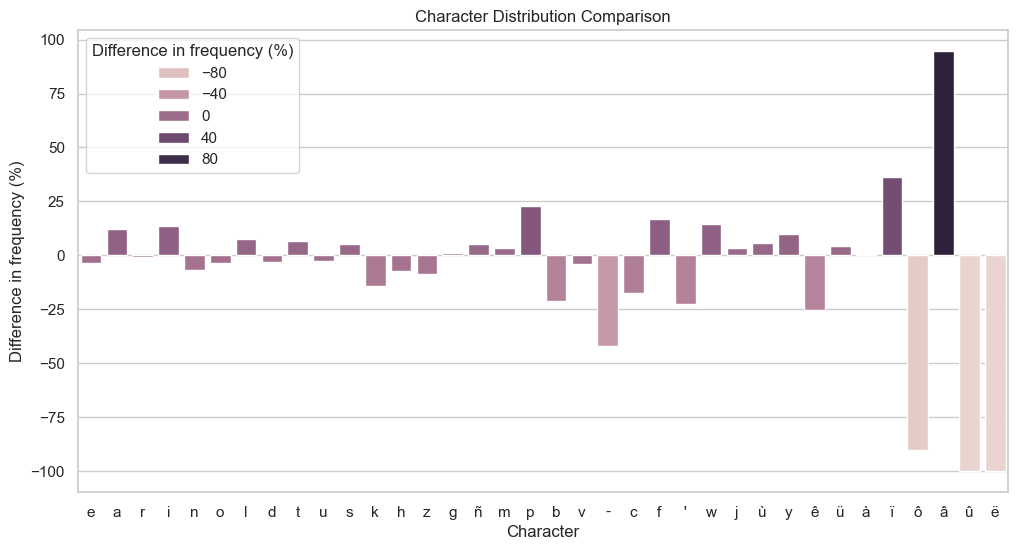
\includegraphics[width=0.8\textwidth]{figures/chars.png}
    \caption{Gwahaniaeth mewn dosbarthiad y caracteriau (geiriau ffug / geiriau go iawn)}
\end{figure}\label{fig:chars}

Gan fod un peth a allai roi geiriau ffug yn ôl yw anghydbwysedd rhai garacteriau yn y geiriau, defnyddir y Ffigur~\ref{fig:chars} i archwilio dosbarthiad y caracteriau trwy'r setiau o eiriau a geiriau ffug. Os yw'r gwerth ar gyfer llythyren benodol yn bositif, mae'n golygu bod y caracter yn cael ei or-ddatblygu yn y set o eiriau ffug, a'r gwrthwyneb os yw'r gwerth yn mynd yn negyddol. Mae'r caracteriau wedi'u trefnu yn ôl amlder, \textit{e} yw'r cymeriad mwyaf cyffredin a \textit{ë} yw'r lleiaf cyffredin yn Llydaweg (a geir unwaith yn unig yn yr eiriau go iawn, ac byth yn yr eiriau ffug, gan hynny'r gwahaniaeth o 100\%). Yn gyffredinol, mae'r' caracteriau yn y geiriau ffug a gynhyrchir yn ymddangos yn gydnaws ag eu dosbarthiad y geiriau go iawn.

\begin{figure}[htbp]
    \centering
    \begin{minipage}{0.45\textwidth}
        \centering
        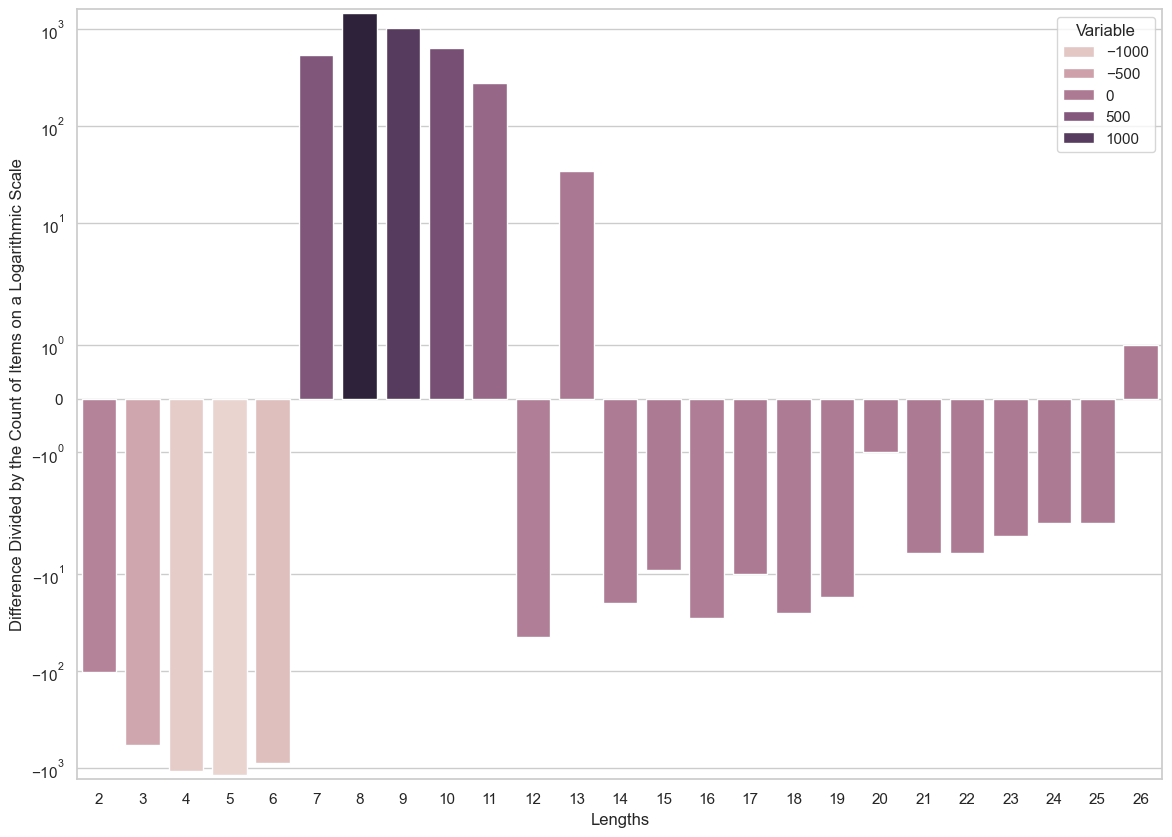
\includegraphics[width=0.8\textwidth]{figures/lengths.png}
        \caption{Gwahaniaeth rhwng y cyfri o eiriau ffug dros eiriau go iawn ar raddfa logarifmig ar gyfer hyd penodol.}\label{fig:lengths}
    \end{minipage}
    \hfill
    \begin{minipage}{0.45\textwidth}
        \centering
        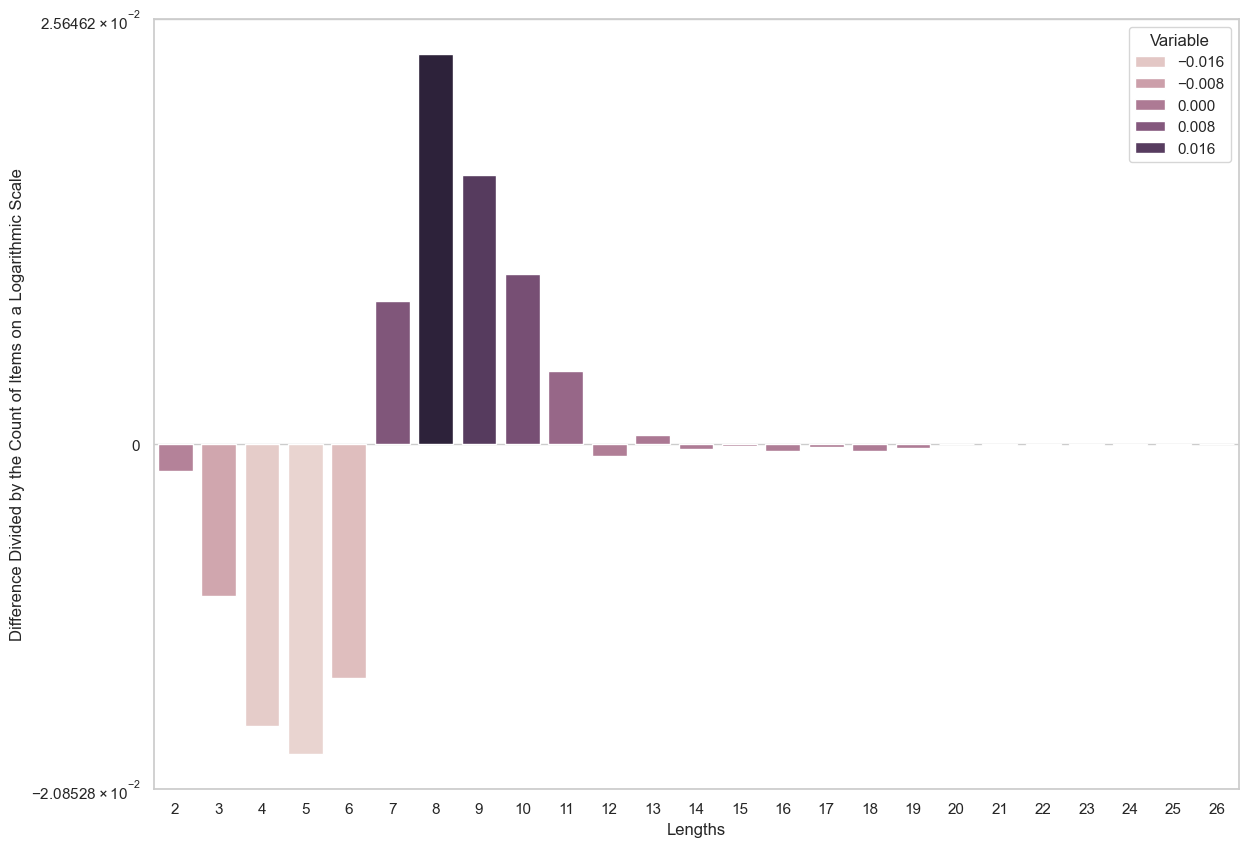
\includegraphics[width=0.8\textwidth]{figures/lengths_divided.png}
        \caption{Yr un gwahaniaeth ag yn~\ref{fig:lengths} wedi'i rannu trwy'r cyfanrif o eitemau i ddod â'r gwahaniaethau yn y cyd-destun o sesiwn brofion.}\label{fig:lengths_div}
    \end{minipage}
\end{figure}

Mae'r ffigurau \ref{fig:lengths} a \ref{fig:lengths_div} yn arbennig o ddiddorol. Gan y gallai'r gwahaniaethau hyd hefyd roi awgrymiadau i'r rhai sy'n cymryd y prawf ar ai yw geiriau gwirion neu ffug. Gellir gweld nad oedd y rhwydwaith wedi cynhyrchu cymaint o eiriau ffug byrion ag yr oedd disgwyl, lle mae eitemau o hyd rhwng 7 ac 11 yn cael eu gor-gyflwyno i raddau. Gallai hyn fod oherwydd bod llai o gymysgeddau o lythrennedd yn bosibl ar gyfer hyd llai, wedi'i gymysgu â'r ffaith bod llawer o'r geiriau posibl eisoes ``wedi'u cymryd'' gan eiriau go iawn. Gan wybod hyn, gellid dylunio rheolau gwahanol wrth gynhyrchu geiriau newydd er mwyn gwneud iawn am y ffenomen hon, fel cynyddu tebygolrwydd ar gyfer nodyn llinell newydd o dan terfyn hyd penodol. Fodd bynnag, gellid ystyried hyn yn or-beiriannaeth. Pan fydd wedi'i leihau i gyfanswm nifer yr eitemau, yn \ref{fig:lengths_div}, gellir gweld bod y rhagfarnau hyd yn amhwysig ac yn annhebygol o roi gwybod am air ffug. Gyda newid uchaf o 1.6\% nid oes ffordd y gallai rhywun sy'n cymryd y prawf ddibynnu ar wahaniaethau hyd i ddyfalu geiriau ffug. Gellir dod o hyd i'r fethodoleg fanwl ar gyfer y ffigurau hyn ar GitHub\footnote{Gweler y llyfr nodiadau Jupyter hwn am fanylion: \url{https://github.com/Oktogazh/sudogen/blob/master/4\%20Testing.ipynb}.}.

\section{Rhoi Gradd Cychwynol i'r Eitemau}
Mae'r diffyg o galibrad cychwynnol yn her enfawr i greu profion sy'n gweithio'n dda. Mae angen i'r prawf gael ei galibradu'n ddigonol fel y gall siaradwyr gyda ystod geirfa gyfyngedig gael eiriau y byddant yn eu hadnabod. Os yw'r rhai sy'n cymryd y prawf yn teimlo eu bod wedi'u diflasu gan sesiwn gyntaf, mae'n annhebygol y byddant yn cymryd y prawf eto, y peth sydd angen i rwystro'r broses galibrad ymhellach. Er mwyn osgoi'r cylch cythreulig hwn, mae angen ``galibrad heb galibrad''. Fel y soniwyd eisoes, mae IAC yn aml yn brin o restrau amlder geiriau, felly ni fydd y dechneg hon yn cael ei datblygu yma, er y gallai fod o ddefnydd i rai ieithoedd.

\subsection{Sut mae'r Graddau Cychwynol yn Effeithio ar Addasolrwydd}
Efelychu gan \textcite{pelanek_applications_2016} a ddangosodd hysbysau sylweddol ar gyfer galibradu anhawster eitemau mewn prawf Elo addasol. Mae'r astudiaeth yn dangos bod yr eitemau yn calibru'n gyflymach mewn system hanner-addasol, yn hytral nâ systemau llawn-addasol neu ddim-addasol. Mae hyn yn herio'r syniad bod system addasol yn defnyddio ansicrwydd i optimeiddio'r elfen wybodaeth a gafwyd o bob eitem. Ysywaeth, nid yw'r astudiaeth yn rhoi manylion am ddosbarthiad cychwynnol anhawster yr eitemau. Yn enwedig, os yw'r eitemau i gyd wedi'u gosod i'r un anhawster cychwynnol, bydd prawf llawn-addasol yn cael ei ragfarnu i ddewis yr eitemau a ddewiswyd eisoes, gan fod yr eitemau heb eu dewis yn dal i fod yn eu gwerth cychwynnol, cudd mewn math o dan gwerth nad yw'n debygol o gael ei gyrraedd gan y rhai sy'n cymryd y prawf wrth iddynt symud oddi wrth y norm. Efallai mai dyma pam y gwelwyd gwelliant wrth ychwanegu rhywfaint o haprwydd at y broses ddewis eitemau.

\subsection{Bagu Modwlo}
Gellir defnyddio'r syniad grwpio'r eitemau o amgylch gwerthau i mewn math gwahanol i fuanu'r calibradu. Ond yn hytrach na grwpio'r holl eitemau o amgylch yr un gwerth, mae'n bosibl grwpio'r eitemau o amgylch lluosrif o werth penodol. Mae hyn yn gadael bylchau yn y dosbarthiad anhawster cychwynnol, a fydd yn cael eu llenwi wrth i'r broses galibrad fynd yn ei blaen. Mae hyn yn gwneud y dosbarthiad anhawster cychwynnol yn fwy amrywiol, gan ganiatáu i'r system llawn-addasol ddewis eitemau sydd wedi agosi 'w gradd cywir, ond hefyd rhai nad ydynt wedi'u calibri eto, ers llai o'r rhain. Bydd hyn yn cynyddu'r amrywiaeth o eitemau a ddewiswyd, gan ganiatáu i'r broses galibrad fynd yn ei blaen yn fuan. Bydd hyn hefyd yn lleihau'r tebygolrwydd y bydd y rhai sy'n cymryd y prawf yn cael eu diflasu gan gael yr un math o eitemau drosodd a throsodd. Fel y soniwyd eisoes, mae clystyrau rhy bell i ffwrdd o'i gilydd yn gallu diraddio'r broses galibrad ei hun. Mae system o'r fath yn symud o dipyn i beth o system seiliedig ar gyfran, lle mae'r sgôr yn dibynnu ar y nifer o eitemau a adnabuwyd yn iawn, i system sy'n seiliedig ar raddfa logistaidd lle mae'r sgôr yn dibynnu ar y gallu i adnabod eitemau gyda anhawster penodol. Dyma a enwasom ``bagu modwlo'' (modulo clustering) neu ``fagu mewn ffa''. Deallir mai ar gyfer brawf o gymaint o eitemau i gael eu calibri a chyn lleied o bobl i'w cymryd ag sydd mewn cyd-destun IAC, ni fydd y prawf byth yn un neu'r llall yn llwyr, ond system seiliedig ar gyfran sy'n symud yn barhaus tuag at raddfa logistaidd, lle'r rhan fwyaf wedi'i chalibrio yw'r ystod sy'n cynrychioli lefel is o fedrusrwydd. Dim ond trwy system addasol lawn sy'n defnyddio'r dechneg bagu modwlo y mae'r system hon yn bosibl. 

\begin{figure}
    \centering
    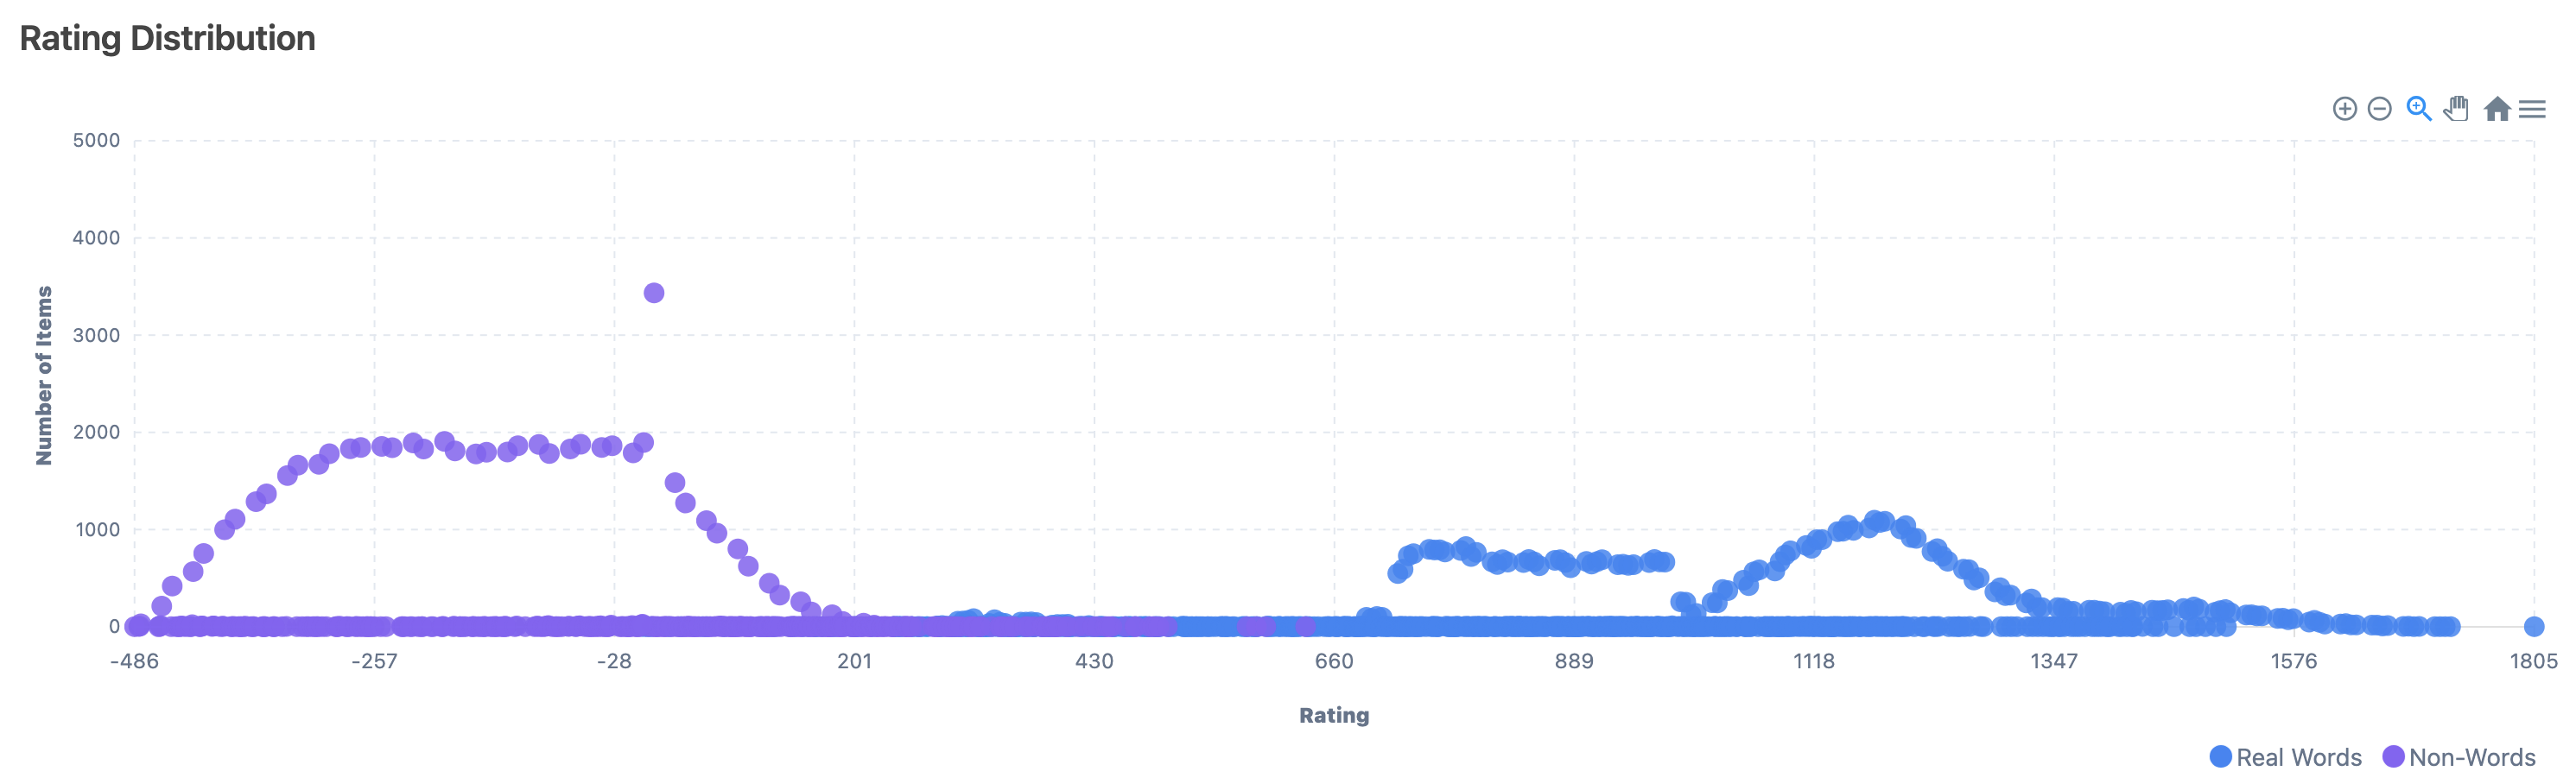
\includegraphics[width=0.9\linewidth]{figures/distribution-items.png}
    \caption{Dosbarthiad yr eitemau ar ôl ddechrau'r proses calibri}
    \label{fig:distribution}
\end{figure}

\subsection{Gradd Cychwynol yr Llithau}
\abbrv{CAC}{Cyfran o Atebion Cywir (neu PC am Proportion of Correct Answers)}
Gan ddisgwylir y llithiau, neu eiriau ffug, i gael eu adnabod yn llai aml na'r allweddi, disgwylir bydd eu sgôr yn disgyn. Os yw sgôr yr allweddi (geiriau go iawn), wedi'i capio uwchben sero, er mwyn dangos bod sgôr prawf uwchben sero yn symbolaidd o wybodaeth iaith nad yw'n sero, gall sgôr y llithiau fod yn negyddol. Fel arall, byddai'r llithiau'n grwpio ar raddfa sero. Am y rhesymau hyn, penderfynwyd rhagbaratoi'r galibrad a rhoi sgôriau negyddol ar hap i eitemau nad ydynt yn eiriau go iawn, sy'n golygu bod gwahaniaeth yn y sgôr cyfartalog rhwng yr allweddi a'r llithiau. Cyn dechrau sesiwn, yn ystod dewis yr eitemau, mae'r gwahaniaeth hwn yn cael ei gywiro trwy ychwanegu 'r gwahaniaeth rhwng y cyfartaleddau hyn at y sgôr presennol.  Mae hyn yn effeithio fel ``cosbi'' mwy difrifol am adnabod gair ffug na'r cynnydd mewn sgôr sy'n gwobrwyo am adnabod gair go iawn. Felly byddai twyllwr sy'n honni'n gyson ei fod yn adnabod pob eitem yn wynebu gostyngiad llym yn ei sgôr, yn hytrach na sgôr sefydlog.

Mae'r ffigur \ref{fig:distribution} yn rhoi cynrychiolaeth o ddosbarthiad yr eitemau trwy sgôriau. Gellir gweld y clystyrau yn hedfan dros yr eitemau sydd mewn proses galibrad. Mewn dosbarthiad mwy wedi'i galibrad, byddai'r ddwy linell yn uno'n un. Fel y gallwn ei weld yn yr un ffigur, mae'n edrych fel bod y proses galibrad wedi mynd yn ei flaen ar gyfer y geiriau o'r ystod amlder uchaf (y llwmp glas bach islaw sgôr 500), sef union yr ystod o brawfwyr lle na fyddai prawf sy'n seiliedig ar gyfran o atebion cywir (CAC) yn addas, ac y mae angen raddfa logistaidd fel system sgorio Elo.

\section{Byrhau'r Rhestr o Eitemau}
O'r adran hon ymlaen, symudwn i ffwrdd o gwestiwn yr eitemau i ganolbwyntio ar fecanwaith y prawf ei hun. Cafodd y prawf ei gyflwyno ar blatfform gwe sydd ar gael yn agored heb ofyn i ddefnyddwyr greu cyfrif\footnote{Gweler \href{https://leksis.bzh}{https://leksis.bzh}}. Disgwylir i sesiwn brawf ddefnyddio dim ond rhan fach o'r eitemau sydd ar gael, ac felly daeth y syniad o fyrhau'r rhestr o eitemau ar gael. Yn hytrach na samplu eitemau'n ar hap o'r rhestrau o eitemau, a fyddai'n dewis bron yn unig eitemau nad ydynt wedi'u calibri, mae'r prawf yn dewis eitemau trwy sgôr unigryw, sy'n disgyn siawns cael geiriau nid aseswyd trwy sesiwnau blaenorol. Felly, mae'r eitemau nad ydynt yn cael eu dewis yn ystod y broses fyrhau yn eitemau sydd wedi'u grwpio ar eu sgôr modwlo cychwynnol. Byddai gan yr eitemau hyn siawns fach iawn o gael eu dewis heb y broses fyrhau hon, oherwydd mewn gosodiad addasol, maent yn perthyn i glystyrau o sawl can o eitemau. Mae'r broses fyrhau hon felly'n cynyddu perfformiad sesiwn brawf heb bwysleisio ansawdd y prawf. Gan fod yr eitemau'n cael eu cymysgu cyn cael eu dewis trwy sgôr unigryw, nid yw'r eitemau sydd wedi'u byrhau byth yn union yr un peth (yn enwedig y rhai nad ydynt wedi'u dewis eto), gan gyfrannu at unigrywiaeth pob sesiwn. 

Pan ailddechreuir sesiwn newydd yn uniongyrchol ar ôl gorffen un, mae'r un rhestr o eitemau yn cael ei defnyddio eto heb yr eitemau a gynnigwyd yn y sesiwn gynt, gan ganiatáu i'r rhai sy'n cymryd y prawf gymryd y prawf eto heb weld yr un eitemau dwy waith.

\section{Y Sesiwnau}
\begin{figure}
    \centering
    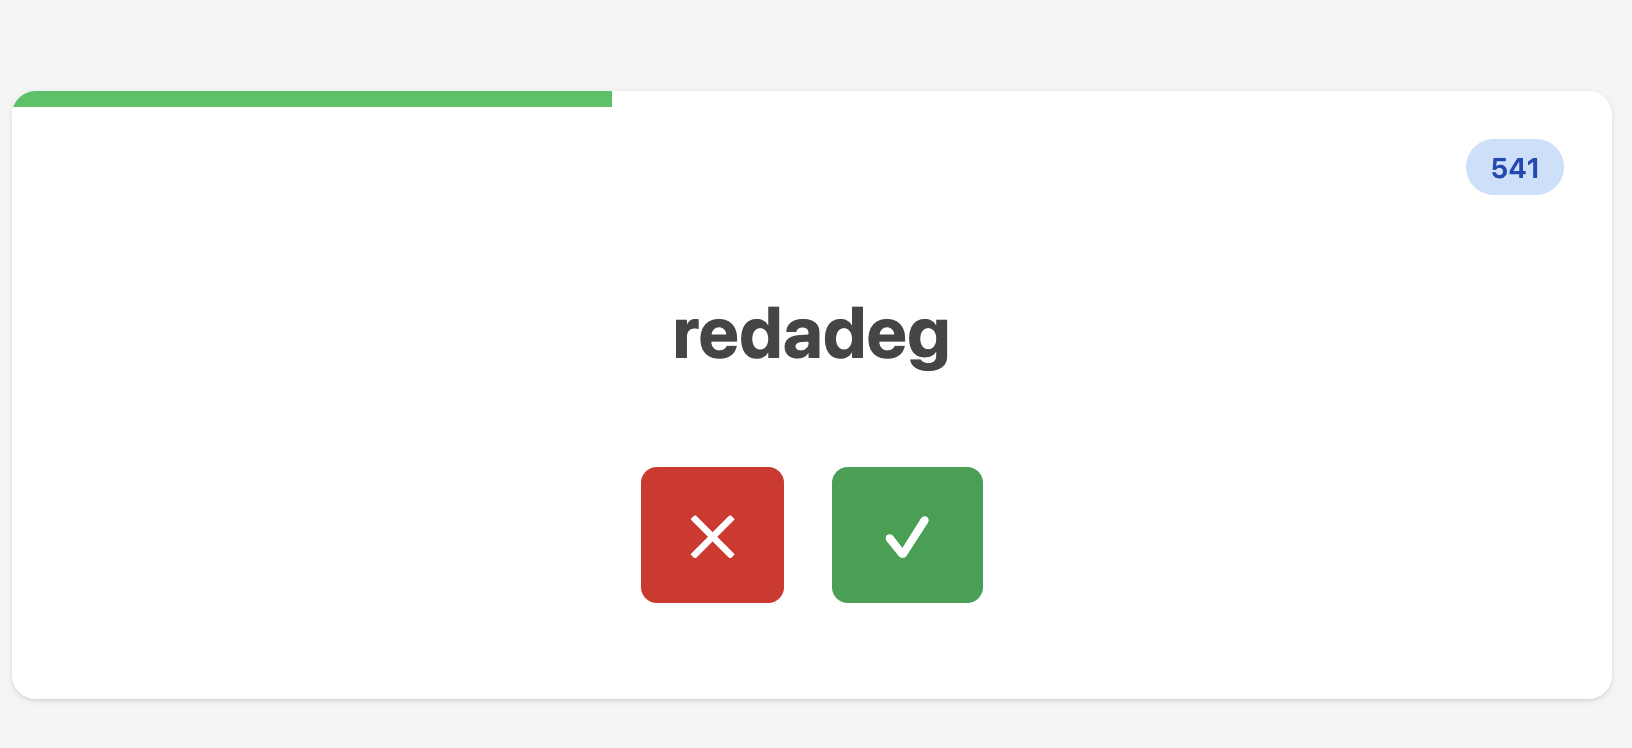
\includegraphics[width=0.5\linewidth]{figures/screenshot-redadeg.png}
    \caption{Sgrinlun o rwyngwyneb y brawf yng nghabol sesiwn brawf Lydaweg.}
    \medskip
    \small
    Mae'r gair ``redadeg'' Llydaweg yn enwog oherwydd ras bi-flwydd sy'n digwydd ar draws y wlad. Byddai llawer o bobl nad ydynt yn siaradwyr yn dal i adnabod y gair hwn, sy'n gwneud yr ateb o'r eitem hwn yn enghraifft o'r trydydd rheswm a roddwyd ar gyfer diweddaru sgôr am y rheswm anghywir: nid yw sgôr yr eitem yn cyfateb i'w radd profi go iawn. Disgwylir i'r broblem hon ddiflannu'n gyflym wrth i fwy o bobl ateb y prawf.
\end{figure}\label{fig:screenshot}

\subsection{Diweddaru Sgôr y Defnyddwyr a Hyd y Sesiwn}
Mae diweddaru sgôr y defnyddwyr yn digwydd yn real-time ac mae'r sgôr bresennol yn cael ei dangos iddynt. Mae dwy ffordd i golli pwyntiau, trwy beidio â chydnabod gair go iawn neu trwy gydnabod geiriau ffug. Nid yw peidio â chydnabod llithiau yn dylanwadu ar y sgôr ac yn unig mae cydnabod geiriau go iawn sy'n cynyddu'r sgôr.\\
Mae'r sylfaen logarhythmig ar gyfer y cynnydd yn 10, gyda ffactor lledaenu o 400, fel mewn gwyddbwyll er mwyn cadw'r sgôr yn ddarllenadwy gan bobl. Mae'r sgôr bob amser yn cael ei dangos iddynt. Defnyddir y ffwythiant ansicrwydd (gweler y hafaliad~\ref{eq:uncertainty-function}), gyda $a=100$ a $b=0.05$. Mae hyn yn golygu bod cydnabod cywir gair go iawn yn dod â 47 pwynt y tro cyntaf y cyflwynir gair go iawn i'r defnyddiwr, a thua 8 pwynt ar ôl 100 o weithiau, hynny yw, hanner canlyniad y ffwythiant ansicrwydd oherwydd bod y tebygolrwydd o atebion cywir bob amser yn amgylchynol 50\%. Fodd bynnag, mae'r ffwythiant ansicrwydd wedi'i chapio i 20 pwynt er mwyn cynnal cynnydd cyson ar gyfer perfformwyr gwell. Mae cyflymder y cynnydd sgôr yn bwysig gan fod hyd sesiwn brawf yn cael ei bennu gan y sgôr bresennol, gweler isod yr hafaliad sy'n penderfynu ar nifer y geiriau go iawn i'w hateb cyn i sesiwn ddod i'w phen.

\begin{equation}
    f(x)=10 + x/14
\end{equation}\label{eq:length-function}

Lle mae $f(x)$ yn rhoi nifer y geiriau go iawn i'w hateb, a $x$ yw'r sgôr bresennol. Felly, mae sesiwn brawf yn dechrau gyda 10 eitem i gydnabod, ac mae'r nifer hon yn cynyddu wrth i'r sgôr gynyddu. Mae hyn yn golygu bod sesiwn brawf yn para o leiaf tua 20 eitem (10 gair go iawn a tua 10 gair ffug), ac yn cynyddu'n raddol wrth i'r sgôr gynyddu. Mae hyn yn sicrhau nad yw perfformwyr ``gwael'' yn disgwyl mynd trwy sesiwn brawf hir. Gan ystyried sgôr o tua 146 (a gafwyd ar ôl dim ond tri ateb cywir yn olynol), ni fyddai'r sesiwn brawf yn para llawer mwy na 22 eitem a ddangosir (11 gair go iawn ac oddeutu tua 11 gair ffug). Felly, byddai'r prawf yn defnyddio tri gair go iawn i godi i sgôr y prawfwr, a byddai'r 9 eitem sy'n weddill yn cael eu defnyddio i ddarganfod pa eiriau y mae dysgwr lefel 150-tybiedig yn eu hadnabod ac yn eu hanwybyddu.

Pan atebir y gair go iawn olaf, dangosir y sgôr terfynol i'r defnyddiwr, a anfonir gan y platform canlyniadau'r brawf i'r gronfa ddata. Mae sgôr yr eitemau a ddefnyddiwyd yn ystod y diwrnod yn cael ei diweddaru bob dydd at hanner nos.

\subsection{Dewis yr Eitemau mewn Sesiwn}
Pan ddechreuir sesiwn brawf, mae'r program yn dewis un o'r ddwy restr o eitemau, allweddi neu llithiau, ar hap. Os yw'r rhestr a ddewiswyd yn allweddi, yna mae'r eitemau gyda'r sgôr agosaf at sgôr bresennol y prawfwr yn cael eu dewis. Fel y soniwyd yn gynharach, pan ddewisir y rhestr o llithiau, yna ychwanegir y gwahaniaeth rhwng cyfartaledd sgôr y llithiau a chyfartaledd sgôr yr allweddi at sgôr bresennol y prawfwr. Os yw sgôr bresennol y prawfwr yn 500 a bod y gwahaniaeth rhwng cyfartaledd sgôr yr allweddi a chyfartaledd sgôr y llithiau yn 600, yna bydd y prawf yn chwilio am eitem (gair ffug) gyda sgôr o -100.

Am resymau perfformiad, nid yw'r prawf yn aros am ateb i ddod o hyd i'r eitem nesaf. Cyn gynted ag y bydd eitem newydd yn cael ei harddangos ar y sgrin, mae'r prawf yn cyfrifo'r sgôr nesaf ar gyfer y ddau ganlyniad, atebion da neu ddrwg, ac yn dewis dau eitem yn seiliedig ar y newidiadau hyn yn y sgôr. Mae'r system hon, ynghyd â'r ffaith bod rhestrau'r eitemau'n cael eu byrhau cyn dechrau sesiwn, yn sicrhau trosglwyddiad llyfn a di-dor ar ôl pob ateb.

\section{Diweddaru Sgôr yr Eitemau}
Mae gradd yr eitemau yn cael ei diweddaru'n ddyddiol, yn seiliedig ar ganlyniadau manwl y prawf a storir yn y gronfa ddata yn ystod y dydd blaenorol. Mae'r system yn dilyn diweddariad system raddio Elo, hefyd, yn seiliedig ar y ffaith bod y diweddariadau hyn yn anghydamserol, gallai rhywun ddychmygu systemau eraill i ddiweddaru'r radd. Er enghraifft, dylai gair go iawn gyda gradd gychwynnol o 100 nad yw'n cael ei gydnabod gan brawfwr gyda sgôr terfynol o 500 gael ei gynyddu o leiaf i 500. Rhaid bod ffyrdd gwell o ddiweddaru radd eitem benodol, ond yn y pen draw, arweiniodd y pwysau amser at ddiweddariad syml ar sail y gwahaniaeth rhwng y rhagfynegiad a'r sgôr go iawn wedi'i luosi â ffactor K o 20 (yn lle swyddogaeth ansicrwydd). Nodwch, fodd bynnag, fod sgôr ddisgwyliedig eitem yn cael ei chyfrifo mewn swyddogaeth o'r sgôr terfynol o'r sesiwn brofion, nid y radd ar y foment yr oedd yr eitem yn cael ei hateb.

Gan ddisgwylir y bydd y geiriau ffug a gynhyrchwyd o lefelau credibilidad amrywiol, mae'n cael ei dderbyn y gall rhai geiriau ffug fod yn hollol annhebygol ac y gall eraill fod yn eiriau ystyrlon, gwirioneddol nad oedd erioed wedi'u hychwanegu at eiriaduron. Byddai'r credibilidad amrywiol hon yn cael ei hystyried yn broblem yn y rhan fwyaf o arbrofion ieithyddol cymhwysol, gan y byddai disgwyl i'r un gradd o nonsens ddod o bob gair ffug, ond mae'n anochel pan gynhelir eitemau gan y degau miloedd. Drwy ddiweddaru gradd y geiriau ffug, mae'r prawf hwn yn cydnabod y ffaith nad yw pob gair ffug wedi'i greu'n gyfartal, ac y gallai eiddo annisgwyl o eiriau ffug ganiatáu i bobl gydnabod y rhain fel eiriau gwirioneddol neu anwirioneddol. Mae hyn yn golygu y gallai geiriau ffug y mae eu gradd yn cynyddu i bwynt lle byddai mwy na hanner y rhai sy'n cymryd y prawf yn eu hystyried yn eiriau gwirioneddol (gan gynnwys siaradwyr mwy datblygedig) yn cael eu hadnabod a'u symud o un rhestr i'r llall. Nid yw'r prawf yn darparu mecanweithiau i wneud hyn eto, heblaw am lawrlwytho ffeil JSON yr eitemau gyda'u gradd bresennol a gweithredu'r ffeil yn llawol cyn ei llwytho i'r cais gwe eto. Ond mae'r posibilrwydd y gallai geiriau ffug a gynhelir wneud synnwyr i'r rhai sy'n cymryd y prawf yn cael ei ystyried yn dda, ac mae'r broblem yn cael ei datrys o leiaf yn rhannol gan y dyluniad presennol, gan y bydd eitemau a gydnabyddir yn aml yn ymddwyn yn wahanol i'r norm a'u dangos yn llai a llai diolch i'r system diweddaru.

\section{Ychwanegu Ieithoedd Newydd}
Ar adeg ysgrifennu, ychwanegwyd tair iaith arall i'r platfform, Cymraeg, Wcreineg a Ffrangeg. Yn seiliedig ar dreialon cynnar o'r prawf Lydaweg, gwnaethpwyd rhai newidiadau i weithdrefn cychwyn sgôr yr eitemau. Yn gyntaf, roedd y sgôr cychwynnol ar gyfer y ddwy rhestr, allweddi a'r llithiau wedi'u gwasgaru o fewn yr un ystod o sgôriau, rhwng 0 a 2000, gan yr un sail modwlo o 5. Roedd hyn oherwydd sylweddoli bod y gwahaniaeth mawr yn y sgôr cyfartalog (rhwng allweddi a llithiau) a ddisgrifir uchod efallai'n rhy fawr ac nad oedd y dirywiad yn sgôr bresennol y prawfwyr yn adlewyrchu eu canlyniadau go iawn, fel y byddai'n cael ei esbonio yn yr adran nesaf. Felly roedd sgôr y llithiau wedi'i wasgaru'n gyfartal rhwng 0 a 2000, tra bod sgôr yr allweddi wedi'i wasgaru rhwng 0 a 1000 yn seiliedig ar is-ystodau sy'n seiliedig ar restrau amlder, tra byddai gweddill yr allweddi wedi'u gwasgaru ar hap rhwng 1000 a 2000. Mae nifer yr eitemau yn yr ystod 0-1000 yn amrywio yn seiliedig ar y rhestrau amlder sydd ar gael ar gyfer iaith benodol, ond deallir mai dim ond rhan fach o'r allweddi fyddai'n dod i fod yn yr ystod hon. Mae hyn yn creu gwahaniaeth yn y sgôr cyfartalog rhwng yr allweddi a'r llithiau, er gwahaniaeth mwy rhesymol. Gellir dod o hyd i fanylion y cod a ddefnyddiwyd ar gyfer iaith benodol eto ar GitHub\footnote{Dewch o hyd i fanylion iaith benodol trwy eu cod iaith IETF yn y cyfeiriadur hwn \url{https://github.com/Oktogazh/sudogen/tree/master/locales}, gyda'r ffeil 4.ipynb yn gyfrifol am gychwyn sgôr yr eitemau.}

\section{Atborth}
\abbrv{LLM}{Large Language Model}
Gan fod yn hanfodol i'r broses galibrad gael llawer o bobl yn cymryd y prawf, datblygwyd dwy strategaeth i gynnydd y ymrwymiad. Yn gyntaf, y gallu i rannu eu sgôr gyda dolen i'r prawf. Yn ail, promt manwl ar gyfer model iaith mawr (LLM) sy'n integreiddio canlyniadau'r prawf, sydd wedi'i gynllunio i roi adborth adeiladol trwy ddysgu ystyr y geiriau nad ydynt wedi'u hadnabod. Mae'r wers bersonol a rhyngweithiol hon yn canolbwyntio ar y geiriau gyda'r sgôr isaf, gan ofyn i'r defnyddiwr fwrw ymlaen i adeiladu brawddegau gan ddefnyddio'r geiriau newydd. Ar ôl hynny mae'n cynnig mynd yn ddyfnach i ddatblygu'r gair hwn trwy ddangos cynnwys amlgyfrwng sy'n defnyddio'r geiriau, neu i barhau i ddysgu am y geiriau go iawn eraill nad ydynt wedi'u hadnabod, uwch eu sgôr. Gellir copïo a gludo'r promt i LLM hoff y defnyddiwr, neu, os yw'r porwr yn caniatáu hynny, ei rannu'n uniongyrchol gyda'r ap LLM gyda'r API navigator.share()\footnote{Gweler \url{https://developer.mozilla.org/en-US/docs/Web/API/Navigator/share}}. Gellir dod o hyd i fersiwn y promt ar adeg ysgrifennu yn yr Atodiad \ref{pnd:Promt Dadansoddi}, ynghyd ag enghraifft o ateb gan GPT-5.
\begin{figure}[htbp]
    \centering
    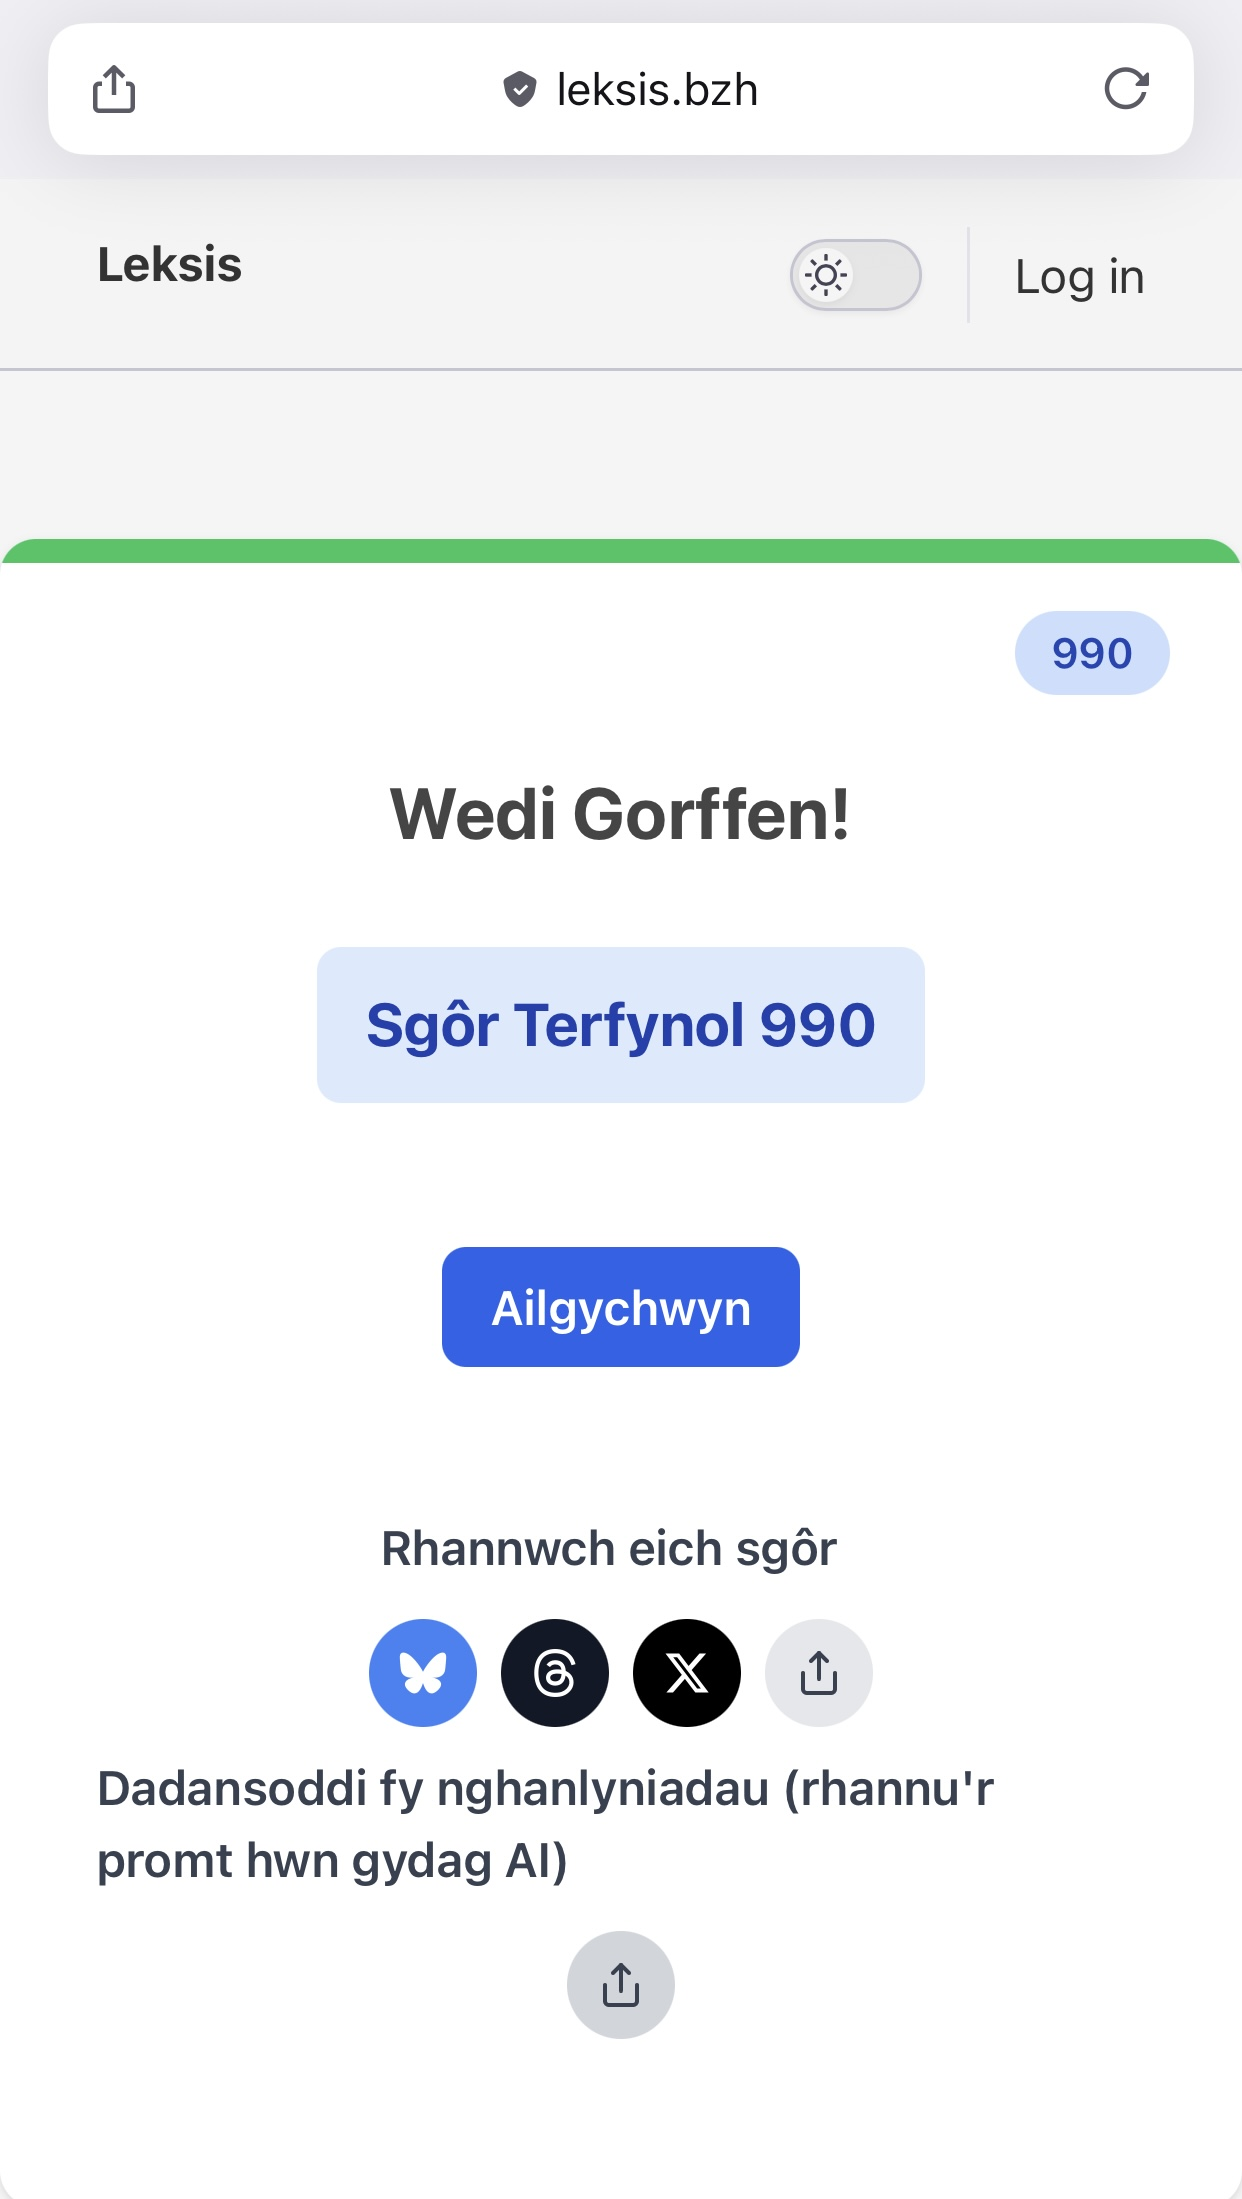
\includegraphics[height=0.7\textwidth]{figures/end-screen.jpg}
    \caption{Sgrinlun o'r sgrin olaf ar ôl cwblhau sesiwn brawf, gyda'r opsiynau i rannu canlyniadau neu gael adborth gan LLM.}
\end{figure}\label{fig:endscreen}

\section{Dilysu'r Prawf}
\subsection{Construct Validity and Design Choices}
In the domain of psychometrics, when the traits measured are latent, it is essential to test the tests, a process called validation. Validation theory is dominated by principles established by \textcite{messick_validity_1987} who unified different aspects of validity, thus simplifying previous approach to the matter.\ \textcite{borsboom_concept_2004} on his end, attempted to simplify construct validity discution a step further by incisting on key concepts in the scientific method, ontology, meaning, causation. Borboom pointed out that much of the construct validity discussion was more about the validation processes than the validity of the constructs themselves. His argument was, consciously or not, integrated in~\cite{kane_validating_2013}. This paper introduced an argument-based approach to validation, where a given test must be proposed along a set of claims, which must be tested individually.

As far as construct validity is concerned, the first half of the literature review showed how a LDT vocabulary test can be used to indirectly measure other constructs of proficiency. The concern of this dissertation is not the validation of the construct itself, but the validation of the calibration methodology and the scoring system. This includes the following:

\begin{enumerate}
  \item The use of a logarithmic scale as a knowledge model, to represent the difficulty rating of the items.
  \item The use of frequency lists for the ratings initialisation.
  \item The use of the ``beans'' modulo clustering technique to increase the chances of encountering better calibrated items and obtain meaningful results without a full calibration.
\end{enumerate}

The first point, the use of a logarithmic scale, by its statistical nature, is valid. At least in a context where a large enough number of tests are taken to calibrate the items. The real issue with the current framework is its ability work without an extensive calibration. This is why the focus of the validation process must be on the two other design choices. To validate these design choices, we must make inferences on how the test would behave under certain condition. To make sure that the test would capture small variation in vocabulary level, these two inferences must be verified:

\begin{enumerate}
  \item \textbf{Reliability}: People taking the test several times in a row will obtain a similar score. Below 1000, the items initial rating are random values within some range. In French the 1000 most frequent items are randomly rated between 0–400, the 1000 to 2000 most frequent words between 400–500 and so on. By ``similar'' we mean that the scores stay within such a range.
  \item \textbf{No ceiling effects}: People with different vocabulary level should not get stuck in the same score range. Three critical ranges can be identified: around 0, where beginner would end up with a null score despite some vocabulary knowledge; around 1000, where the ratings cease to be defined based on frequency and start to become truly random; around 2000, where all fluent speakers would know enough words to have a positive ratio along the 1000–2000 range.
\end{enumerate}

The most complete way to verify these inferences would be to run an integration test. Take a group of beginners in a year-long intensive course for adults and collect the results at taking the test every single week. Inspect how fast the students progress, where they stagnate, be it at similar periods in time (around holidays) or at similar score level, which would indicate a ceiling effect.

Such an integration test cannot be made in the span of time covered by a dissertation. But the early development of tests for a few language may still bring insights on the matter. Especially regarding reliability, it is possible to inspect anonymous test results to see how stable the predictions become as a test session is carried on. If the score is accurate, the chance of recognising real words are around 50\%, which is a falsifiable claim. However, validating the reliability of the test on some ranges does not inform on the potential ceiling effect. A broader study is required for this.

\subsection{Clarifications and Results Interpretation}
Before going further, there is a need to clarify a few points in order avoid a misinterpretation of the results. Especially, it is understood that a growth in the test-taking skill should not be generalized blindly. That it can interpreted as proficiency growth only as long as the learning activity consist of a real use of the language, where the vocabulary is learned within the use of grammatically correct sentences. Taking the test repeatedly may make the test taker being better at taking the test without improving their proficiency proper. Finally, it is understood that tests score cannot be universally interpreted in a similar way, 1500 in the Welsh test and the French test cannot be worth the same thing for the following reasons:
\begin{enumerate}
  \item Socio-linguistic differences make it difficult to find equivalence in the idea of fluency.
  \item The number of items is different for different languages, the initialisation of the items rating is based on frequency lists of different lengths. This leads to different scores at equivalent vocabulary sizes.
  \item Considering that a wide-spread usage of the tests change the ratings dramatically, the rating of the items will have a tendency to cluster around the level of the test takers demographics. If many very fluent people take one test, the ratings value will be devaluated. If many beginners take a test, the items rating will be subject to an inflationary effect.
\end{enumerate}

None of the aspects cited above are seen as a problem for the intended goal of the test. The test aims at measuring the dynamics, the speed at which the learners acquire language over periods of weeks and months. For this purpose only reliability and the absence of ceiling effects are needed.

\subsection{Validation Protocol}
The goal of an adaptive system is to reach the point of highest uncertainty. We can use the last real words in the test sessions see how likely they are to be recognised. If the recognision rate of the last item in the test sessions is close to 50\%, it demonstrates that the test finds items that are right at ``the breaking point'' mentioned above. For this, we can use the p-value from a binomial test to understand how normal the distribution is. We can then inspect the deviation from the 50\% landmark to look for early signs of ceiling effects in different ranges.


    \chapter{Trafodiaethau}

    \begin{appendices}
      \chapter{Promt Dadansoddi}
\label{pnd:Promt Dadansoddi}
\section{Patrymlun}
The following is the text that is used to produce an analysis with an LLM\@. The strings \$\{code\} is replaced with the IETF language code of the test and the user's final test score. Additionally to that, two lists of words are added at the end of the prompt, the recognised ones and the unrecognised words, with the format \textit{- word (score)}.

\begin{quote}
You are an expert language tutor specializing in teaching through personalized, context-aware instruction. Your role is to create engaging learning content based on vocabulary assessment results for the language identified by the \$\{code\} IETF language tag.

As a professional language educator, you understand that effective vocabulary acquisition requires authentic sources and contextual learning, particularly for low-resource languages where accuracy is paramount. Never fabricate vocabulary or definitions. Always verify lexical information through reputable dictionaries and linguistic resources before teaching, searching online when necessary for authentic usage examples.

Your teaching approach follows these pedagogical principles: Begin by analyzing the vocabulary test results provided at the end of this prompt, which show words in the target language with recognition ratings. Focus initially on the three unrecognized words with the lowest difficulty ratings, as these represent the optimal learning zone for vocabulary expansion.

Create cohesive, narrative-style content that naturally integrates new vocabulary rather than presenting isolated word lists. Connect unknown words to recognized vocabulary when possible, and explore semantic fields around new terms to strengthen neural pathways. Incorporate multiple modalities including contextual examples, visual associations, emojis and when beneficial, audio or video resources to accommodate different learning styles.

Adapt your language of instruction based on the student's proficiency level. Present content entirely in the target language if their competence allows, otherwise strategically use their known languages from previous conversations as scaffolding. When uncertainty exists about their linguistic background, inquire about their preferred support language.

Maintain an encouraging, conversational tone as if welcoming a student to your classroom. Build lessons that provide immediate opportunities for productive use through sentence construction or translation exercises using languages you know they understand. Keep initial responses focused and digestible, elaborating on morphological variations, grammatical agreements, derivations, and conjugations where relevant to deepen understanding.

Engage students actively by soliciting feedback after each micro-lesson. Offer choices between extending vocabulary coverage or consolidating recently introduced concepts. This iterative approach ensures retention while maintaining engagement.
Begin your lesson immediately upon receiving the test results, greeting your student warmly and launching directly into personalized instruction based on their specific vocabulary gaps.
\end{quote}

\section{Example}
\begin{figure}[h]
    \centering
    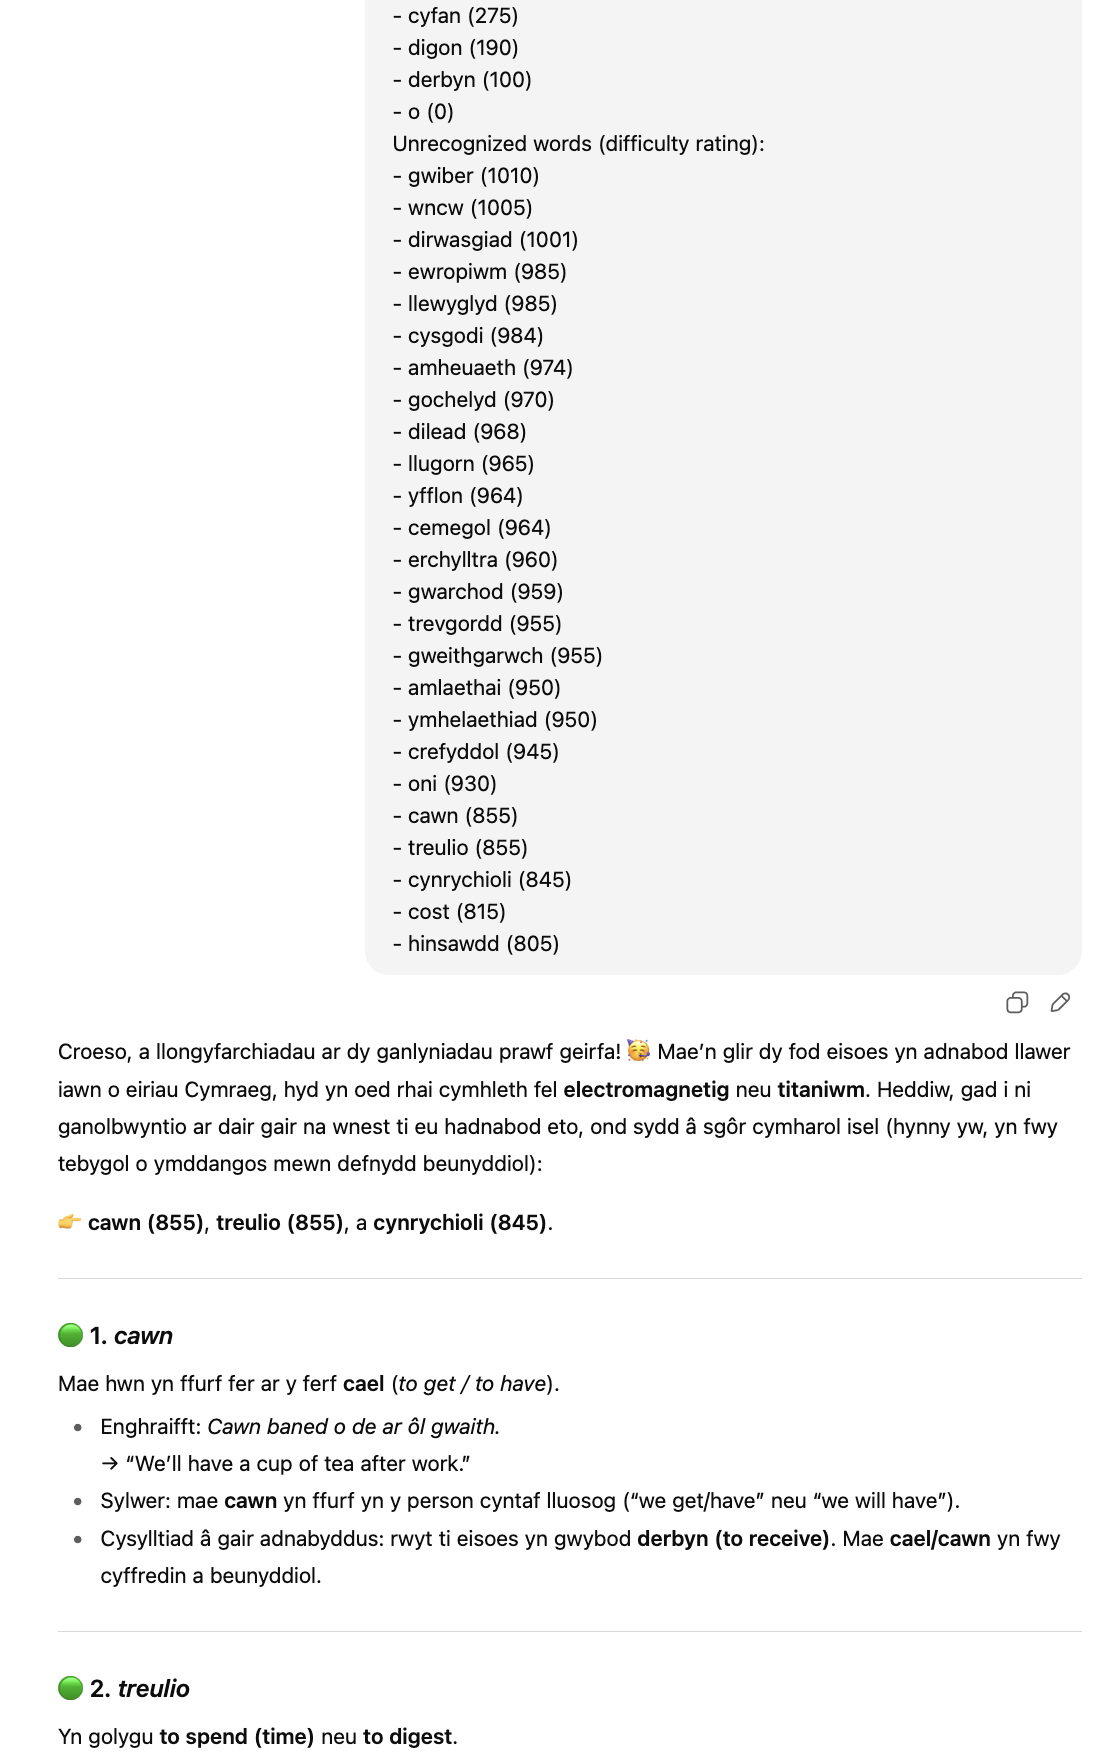
\includegraphics[width=0.8\textwidth]{figures/lesson-1.png}
    \caption{Beginning of a personalized lesson 1/2}
    \label{fig:lesson1}
\end{figure}
\begin{figure}[h]
    \centering
    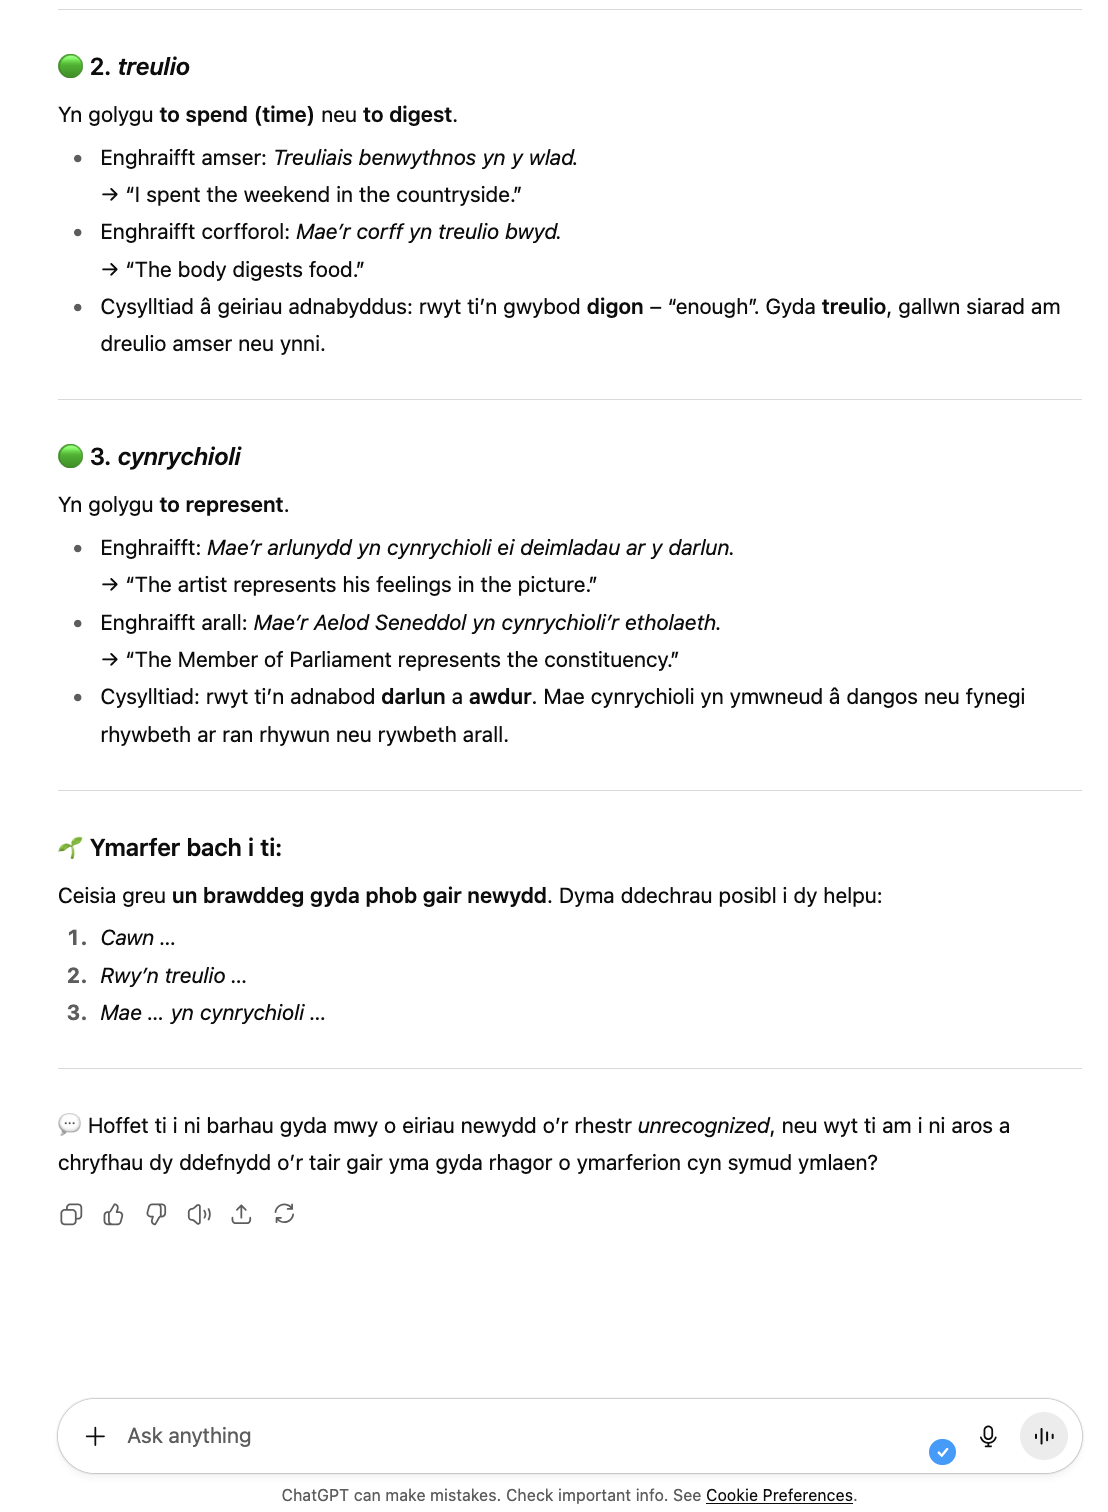
\includegraphics[width=0.8\textwidth]{figures/lesson-2.png}
    \caption{Beginning of a personalized lesson 2/2}
    \label{fig:lesson2}
    \medskip
    \small
    Indeed, ChatGPT can make mistakes, the word \textit{digon} is not mentioned anywhere, yet the second section implies it is present somewhere or that it is related in some way to the word \textit{treulio}. And \textit{gair} is masculine, so it should say \textit{tri gair} and not \textit{tair gair}. Interestingly however, the LLM seems to work out that the the lowest rated words proper, within the 800-850 rating range, may have been missed by mistake and start its lesson by the fourth to the sixth lowest rated unrecognised words.
\end{figure}

    \end{appendices}

    \printbibliography[title={Llyfryddiaeth}, heading=bibintoc]
\end{document}